%\documentclass[handout,dvipsnames,12pt]{beamer} % for the version to send to students
\documentclass[dvipsnames,aspectratio=169]{beamer} % for the version with visual breaks
\usepackage{tikz,xcolor,amsfonts}
\usetikzlibrary{arrows,shapes}
\usepackage[absolute,overlay]{textpos}
\usepackage{multirow}
\usepackage{environ,lipsum}
\usepackage{listings}



\lstset{ 
  language=R,                     % the language of the code
  basicstyle=\scriptsize\ttfamily, % the size of the fonts that are used for the code
  columns=fullflexible,
%  numbers=left,                   % where to put the line-numbers
%  numberstyle=\tiny\color{Blue},  % the style that is used for the line-numbers
%  stepnumber=1,                   % the step between two line-numbers. If it is 1, each line
                                  % will be numbered
%  numbersep=5pt,                  % how far the line-numbers are from the code
  backgroundcolor=\color{Dandelion!15!white},  % choose the background color. You must add \usepackage{color}
  showspaces=false,               % show spaces adding particular underscores
  showstringspaces=false,         % underline spaces within strings
  showtabs=false,                 % show tabs within strings adding particular underscores
  frame=single,                   % adds a frame around the code
  rulecolor=\color{Dandelion!15!white},        % if not set, the frame-color may be changed on line-breaks within not-black text (e.g. commens (green here))
  tabsize=2,                      % sets default tabsize to 2 spaces
  captionpos=b,                   % sets the caption-position to bottom
  breaklines=true,                % sets automatic line breaking
  breakatwhitespace=false,        % sets if automatic breaks should only happen at whitespace
  keywordstyle=\color{RoyalBlue!80!black},      % keyword style
  commentstyle=\color{YellowGreen!60!black},   % comment style
  %stringstyle=\color{ForestGreen}      % string literal style
} 
\lstset{alsoletter={.,_}, morekeywords={cor.test,set.seed,dcor.test,make_tree,sample_gnm,graph,ci.test,qgraph,sample_smallworld,ciTest_table,IsingFit,averageLayout,read.table,install.packages,bdgraph,stepwise,dmod,cmod,ciTest,graph_from_adjacency_matrix,mvrnorm,CondIndTest,as.data.frame,chisq.test,gnm,smallworld,ug,dag,edge,as.igraph,degree,diameter,centrality,cluster,betweenness,at,cptable}
}


\newcommand{\customframefont}[1]{
\setbeamertemplate{itemize/enumerate body begin}{#1}
\setbeamertemplate{itemize/enumerate subbody begin}{#1}
}

\NewEnviron{framefont}[1]{
\customframefont{#1} % for itemize/enumerate
{#1 % For the text outside itemize/enumerate
\BODY
}
\customframefont{\normalsize}
}



%%%%%%%%% BASICS
\usenavigationsymbolstemplate{}

\setbeamertemplate{frametitle}
  {\begin{centering}\smallskip
   \insertframetitle\par
   \smallskip\end{centering}}
\setbeamersize{text margin left=.2cm,text margin right=.2cm} 
\setbeamertemplate{itemize item}{$\bullet$}
\setbeamertemplate{navigation symbols}{}
\setbeamertemplate{footline}[text line]{%
    \hfill\strut{%
        \scriptsize\sf\color{black!60}%
        \quad\insertframenumber/\inserttotalframenumber
    }%
    \hfill
    
}

%%%%%%%%% COLOR THEME

% Define some colors:
\definecolor{asparagus}{rgb}{0.53, 0.66, 0.42}
\definecolor{DarkFern}{HTML}{407428}
\definecolor{DarkCharcoal}{HTML}{4D4944}
\colorlet{Fern}{DarkFern!85!white}
\colorlet{Charcoal}{DarkCharcoal!85!white}
\colorlet{LightCharcoal}{Charcoal!50!white}
\definecolor{Important}{RGB}{234,122,133}
\colorlet{AlertColor}{Melon!30!red}
\colorlet{DarkRed}{red!70!black}
\colorlet{DarkBlue}{blue!70!black}
\colorlet{DarkGreen}{green!70!black}
% Use the colors:
\setbeamercolor{title}{fg=Fern}
\setbeamercolor{frametitle}{fg=Fern}
\setbeamercolor{normal text}{fg=Charcoal}
\setbeamercolor{block title}{fg=black,bg=Fern!15!white}
\setbeamercolor{block body}{fg=black,bg=Fern!15!white}
%\setbeamercolor{block body alerted}{fg=black,bg=Goldenrod!5!white}
%\setbeamercolor{block body example}{fg=black,bg=Fern!15!white}
\setbeamercolor{alerted text}{fg=AlertColor}
\setbeamercolor{itemize item}{fg=Charcoal}
\setbeamercolor{framesource}{fg=gray}
\setbeamerfont{framesource}{size=\tiny}

%%%%% DEFINITIONS

\DeclareMathOperator{\sgn}{sgn}
\DeclareMathOperator{\rank}{rank}
\DeclareMathOperator{\D}{D}
\DeclareMathOperator{\cov}{cov}
\DeclareMathOperator{\var}{var}
\DeclareMathOperator{\tr}{tr}
\DeclareMathOperator{\pa}{pa}
\DeclareMathOperator{\nd}{nd}

\newcommand{\bx}{\mathbf{x}}
\newcommand{\by}{\mathbf{y}}
\newcommand{\C}{\mathbb{C}}
\newcommand{\cC}{\mathcal{C}}
\newcommand{\E}{\mathbb{E}}
\newcommand{\cE}{\mathcal{E}}
\newcommand{\cI}{\mathcal{I}}
\newcommand{\J}{\rm {J}}
\newcommand{\cL}{\mathcal{L}}
\newcommand{\cM}{\mathcal{M}}
\newcommand{\N}{\mathbb{N}}
\renewcommand{\P}{\mathbb{P}}
\newcommand{\Q}{\mathbb{Q}}
\newcommand{\R}{\mathbb{R}}
\renewcommand{\S}{\mathbb{S}}
\newcommand{\cS}{\mathcal{S}}
\newcommand{\cX}{\mathcal{X}}
\newcommand{\cY}{\mathcal{Y}}
\newcommand{\Z}{\mathbb{Z}}
\newcommand{\bs}{\boldsymbol}
\newcommand{\why}{\textcolor{WildStrawberry}{{\textsc{why?}}}}
\newcommand{\indep}{\mbox{\,$\perp\!\!\!\perp$\,}}
\newcommand{\mtp}{{\rm MTP}_{2}}


\def\imagetop#1{\vtop{\null\hbox{#1}}}
\def\house{\hbox{\kern3pt \vbox to12pt{}% 
   \pdfliteral{q 0 0 m 0 5 l 5 10 l 10 5 l 10 0 l 7 0 l 7 5 l 3 5 l 3 0 l f
               1 j 1 J -2 5 m 5 12 l 12 5 l S Q }%
   \kern 13pt}}

%source for images
\newcommand{\source}[1]{\begin{textblock*}{4cm}(8.7cm,8.6cm)
    \begin{beamercolorbox}[ht=0.5cm,right]{framesource}
        \usebeamerfont{framesource}\usebeamercolor[fg]{framesource} Source: {#1}
    \end{beamercolorbox}
\end{textblock*}}

%%% TITLE INFO

\title{Advanced techniques in applied economics}
\subtitle{Modelling with graphs, Lectures 6-10}

\author{Piotr Zwiernik}

\institute{Universitat Pompeu Fabra}

\institute{\begin{center}
  \raisebox{-0.5\height}{
\includegraphics[scale=.27]{LOGOstats.png}}
  \hspace{1mm}
  \raisebox{-0.5\height}{
\includegraphics[scale=.08]{LOGOBSE.jpg}}
\end{center}}


\setbeamercolor{notabene}{fg=black!50!white,bg=Gray!10!white}
\setbeamercolor{important}{fg=red!50!white,bg=red!7!white}
\setbeamercolor{goldbox}{fg=black!50!white,bg=Goldenrod!7!white}
\setbeamercolor{result}{fg=black!60!white,bg=OliveGreen!4!white}
% \begin{beamercolorbox}[wd=\paperwidth,sep=7pt]{important}	
%	%\end{beamercolorbox}


\begin{document}

%\addtocounter{framenumber}{-1}
\begin{frame}[noframenumbering,plain]
  \titlepage
\end{frame}




\section{Bayesian networks and causal discovery}

\begin{frame}[plain,noframenumbering]{}
\begin{center}
	{\Huge \textcolor{DarkRed}{Part 4: Bayesian networks and causal discovery}}
\end{center}
\end{frame}

\subsection{DAGs and their models}

\begin{frame}[plain,noframenumbering]{}
\begin{center}
	{\huge \textcolor{DarkRed}{4.1 DAGs and their models}}
\end{center}
\end{frame}

\begin{frame}{DAG terminology}
\textcolor{blue}{Directed acyclic Graph (DAG)} is a directed graph with no directed cycles.\\[.2cm]
Equivalently, we can order the vertices so that an arrow always goes from smaller to larger vertex.\\[.2cm]
	\alert{parents $\pa(v)$}: nodes $u$ such that $u\to v$ in $G$,\\[.3cm]
	directed path $u\to \cdots \to v$,\\[.3cm]
	path $u\leftrightarrow \cdots \leftrightarrow v$,\\[.3cm]
	\alert{descendants ${\rm de}(v)$} all nodes $u$ s.t. there is a directed path from $v$ to $u$,\\[.3cm]
	\alert{non-descendants $\nd(v)$}: all the other nodes in $V\setminus \{v\}$.\\[.3cm]
	\alert{$v$-structure (immorality)}: \textbf{induced} subgraph of the form $u\to w\leftarrow v$
\end{frame}

\begin{frame}{Example}
DAG from the Chest Clinic Example Lauritzen\& Spiegelhalter (1988). Shortness of breath (dysponea) is the response variable.
	\begin{center}
		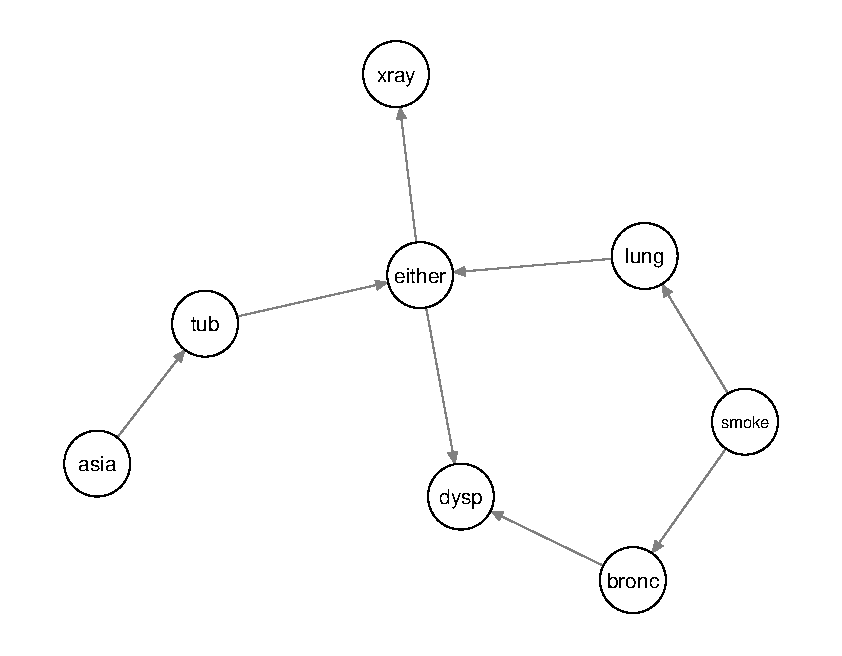
\includegraphics[scale=.5]{pics/chestdag}
	\end{center}
	Give an example of a v-structure. What are the parents of \texttt{either}? Is there a directed path from \texttt{bronc} to \texttt{xray}? Who are the descendants of \texttt{asia}? Who are the non-descendants?
\end{frame}

\begin{frame}[fragile]{d-separation}
	A path $\pi$ from vertex $i$ to vertex $j$ is \alert{blocked} by $S\subset V$ if $\pi$ contains one of the following types of nodes:
	\begin{itemize}
		\item $v\in S$ such that the path looks locally like $\to v\to $, $\leftarrow v\leftarrow$, or $\leftarrow v\to$.
		\item  $v\notin S$ such that $S\subseteq \nd(v)$ and the path looks locally like $\to v\leftarrow$.
	\end{itemize} 
	\bigskip
	
	Two subsets $A$ and $B$ are said to be \alert{d-separated} by $S$ if all paths from $A$ to $B$ are blocked by $S$.
	
	\medskip 
	Package \texttt{bnlearn} has a function \texttt{dsep} to check d-separation:
\begin{lstlisting}
> library(bnlearn)
> chestdag = model2network("[asia][tub|asia][smoke][lung|smoke][bronc|smoke][either|lung:tub][xray|either][dysp|bronc:either]")
> dsep(chestdag, "asia", "xray", c("lung","bronc"))	
[1] FALSE
# the shortest path from asia to xray is not blocked by c("lung","bronc")
\end{lstlisting}
[Mention hierarchical layouts]
\end{frame}

\begin{frame}{DAG models/Bayesian networks}
	Let $G$ be a directed acyclic graph (DAG).\\
	We say that $f(\bs x)$ factorizes according to $G$ if for all $\bs x\in \cX$
	$$
	f(\bs x)\;=\;\prod_{v\in V}f(x_v|\bs x_{{\rm pa}(v)}).
	$$
%	\begin{alertblock}{Chain rule in probability} 
%	For any ordering of the nodes in $V$ we have
%	$$f(\bs x)=f_{v_1}(x_{v_1})f_{v_2|v_1}(x_2|x_1)\cdots f_{v_m|V\setminus m}(x_{v_m}|x_{V\setminus m}).$$
%	\end{alertblock}
%	\vspace{-.5cm}
%	\begin{alertblock}{Important reformulation of conditional independence} 
%$i\indep j|C$ \quad if\quad  
%	$f_{i|C\cup j}(x_i|\bs x_{C\cup j})=f_{i|C}(x_i|\bs x_{C}).$
%	\end{alertblock}
%	\medskip
\begin{beamercolorbox}[wd=\paperwidth,sep=5pt]{important}
	Factorization is equivalent to any of the following Markov properties:
	\begin{itemize}
		\item [(G)] $A\indep B|S$ whenever $S$ d-separates $A$ and $B$.
		\item [(L)] $v\indep \nd(v)|\pa(v)$ for every $v\in G$.
	\end{itemize}
	This results holds with no restrictions on the support of $f$.
\end{beamercolorbox}	
\medskip
We reiterate: $i\indep j|S$ if and only if $S$ \alert{d-separates} $i$ and $i$ in $G$.
\end{frame}

%\begin{frame}{Hierarchical layout}
%ichestdag <- igraph.from.graphNEL(as.graphNEL(chestdag))
%dag <- toVisNetworkData(ichestdag)
%visNetwork(dag$nodes,dag$edges) %>% 
%visEdges(arrows = "from") %>% 
%visHierarchicalLayout() # same as   visLayout(hierarchical = TRUE) 
%\end{frame}

\begin{frame}[fragile]{Belief propagation and inference}
	Belief propagation provides a computationally efficient way to compute various marginal and conditional distributions for a DAG model.\\[.2cm]
First we set up some distribution by specifying terms of the factorization.
	\begin{lstlisting}
library(gRain)
yn <- c("yes","no")
a <- cptable(~asia,values=c(1,99),levels=yn)
t.a <- cptable(~tub+asia,values=c(5,95,1,99),levels=yn)
s <- cptable(~smoke,values=c(5,5),levels=yn)
l.s <- cptable(~lung+smoke,values=c(1,9,1,99),levels=yn)
b.s <- cptable(~bronc+smoke,values=c(6,4,3,7),levels=yn)
e.lt <- cptable(~either+lung+tub,values=c(1,0,1,0,1,0,0,1),levels=yn)
x.e <- cptable(~xray+either,values=c(98,2,5,95),levels=yn)
d.be <- cptable(~dysp+bronc+either,values=c(9,1,7,3,8,2,1,9),levels=yn)
plist <- compileCPT(list(a,t.a,s,l.s,b.s,e.lt,x.e,d.be))
grn1 <- grain(plist) # Graphical Independence Network
grn1c <- compile(grn1)
grn1c <- propagate(grn1c) # at this point probabilistic queries can be asked\end{lstlisting}
\end{frame}


\begin{frame}[fragile]{}
		To compute various joint distributions and conditional distributions of a variable given a subset of variables we run.
\begin{lstlisting}
> querygrain(grn1c,nodes=c("lung","bronc"),type="joint")
     bronc
lung     yes     no
  yes 0.0315 0.0235
  no  0.4185 0.5265
  
> querygrain(grn1c,nodes=c("dysp","asia"),type="conditional")
     dysp
asia        yes        no
  yes 0.4501375 0.5498625
  no  0.4358275 0.5641725
\end{lstlisting}
We can also see what happens when we fix values of some variables. 
\begin{lstlisting}
> grn1c.ev <- setFinding(grn1c,nodes=c("asia","smoke"),states=c("yes","yes"))
> querygrain(grn1c.ev,nodes=c("lung","bronc"),type="joint")
     bronc
lung   yes   no
  yes 0.06 0.04
  no  0.54 0.36
\end{lstlisting}
For examples see: \url{www.bnlearn.com/bnrepository/}
\end{frame}

\begin{frame}[fragile]{Learning distributions from data}
In some special situations the DAG structure can be specified by an expert.\\[.3cm]

	Given data we can then learn the underlying conditional probabilities.
	\begin{lstlisting}
> data("chestSim500",package='gRbase')
> simdagchest <- grain(as.graphNEL(chestdag),data=chestSim500)
> simdagchest <- compile(simdagchest,propagate=TRUE,smooth=.1)
 \end{lstlisting}
	Then inference can be made as explained earlier.
		\begin{lstlisting}
> querygrain(simdagchest,nodes=c("lung","bronc"),type="joint")
     bronc
lung         yes         no
  yes 0.02539682 0.02060318
  no  0.42860318 0.52539682	
 \end{lstlisting}
 Note that the estimated values of the probabilities are close to the truth.
\end{frame}


\begin{frame}[fragile]{Learning the graph}
Learning the underlying DAG from the data is a major problem. \\[.3cm]

\begin{beamercolorbox}[wd=\paperwidth,sep=5pt]{result}
Important links:\\[.2cm]
\textcolor{blue}{\url{annehpetersen.shinyapps.io/causalDisco/}} -- an overview of available methods to learn DAGs in \texttt{R}.	\\[.1cm]
\textcolor{blue}{\url{www.bnlearn.com}} -- an overview of methods in \texttt{bnlearn}.	
	\end{beamercolorbox}

\begin{alertblock}{Example: Coronary artery disease data}
	A cross classified table with observational data from a Danish heart clinic. The response variable is \textcolor{asparagus}{coronary artery disease (CAD)}:
	\begin{lstlisting}
data(cad1,package='gRbase')
cad.bn <- hpc(cad1)
qgraph::qgraph(cad.bn)
# in case you want to exclude some edges
cad.bn.2 <- hc(cad1,blacklist=as.data.frame(matrix(c("CAD","Sex"),1,2)))
\end{lstlisting}
\end{alertblock}
\end{frame}

\begin{frame}{}
\begin{center}
	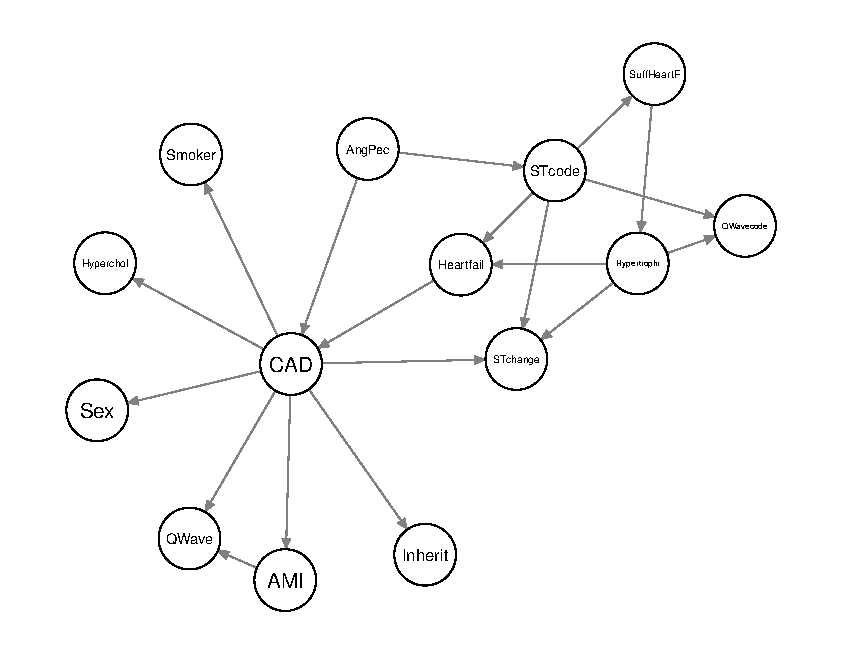
\includegraphics[scale=.7]{pics/cad_hc}
\end{center}
	It is important to incorporate prior knowledge. 
See \url{http://www.bnlearn.com/examples/whitelist/} for details.
\end{frame}

\begin{frame}{}
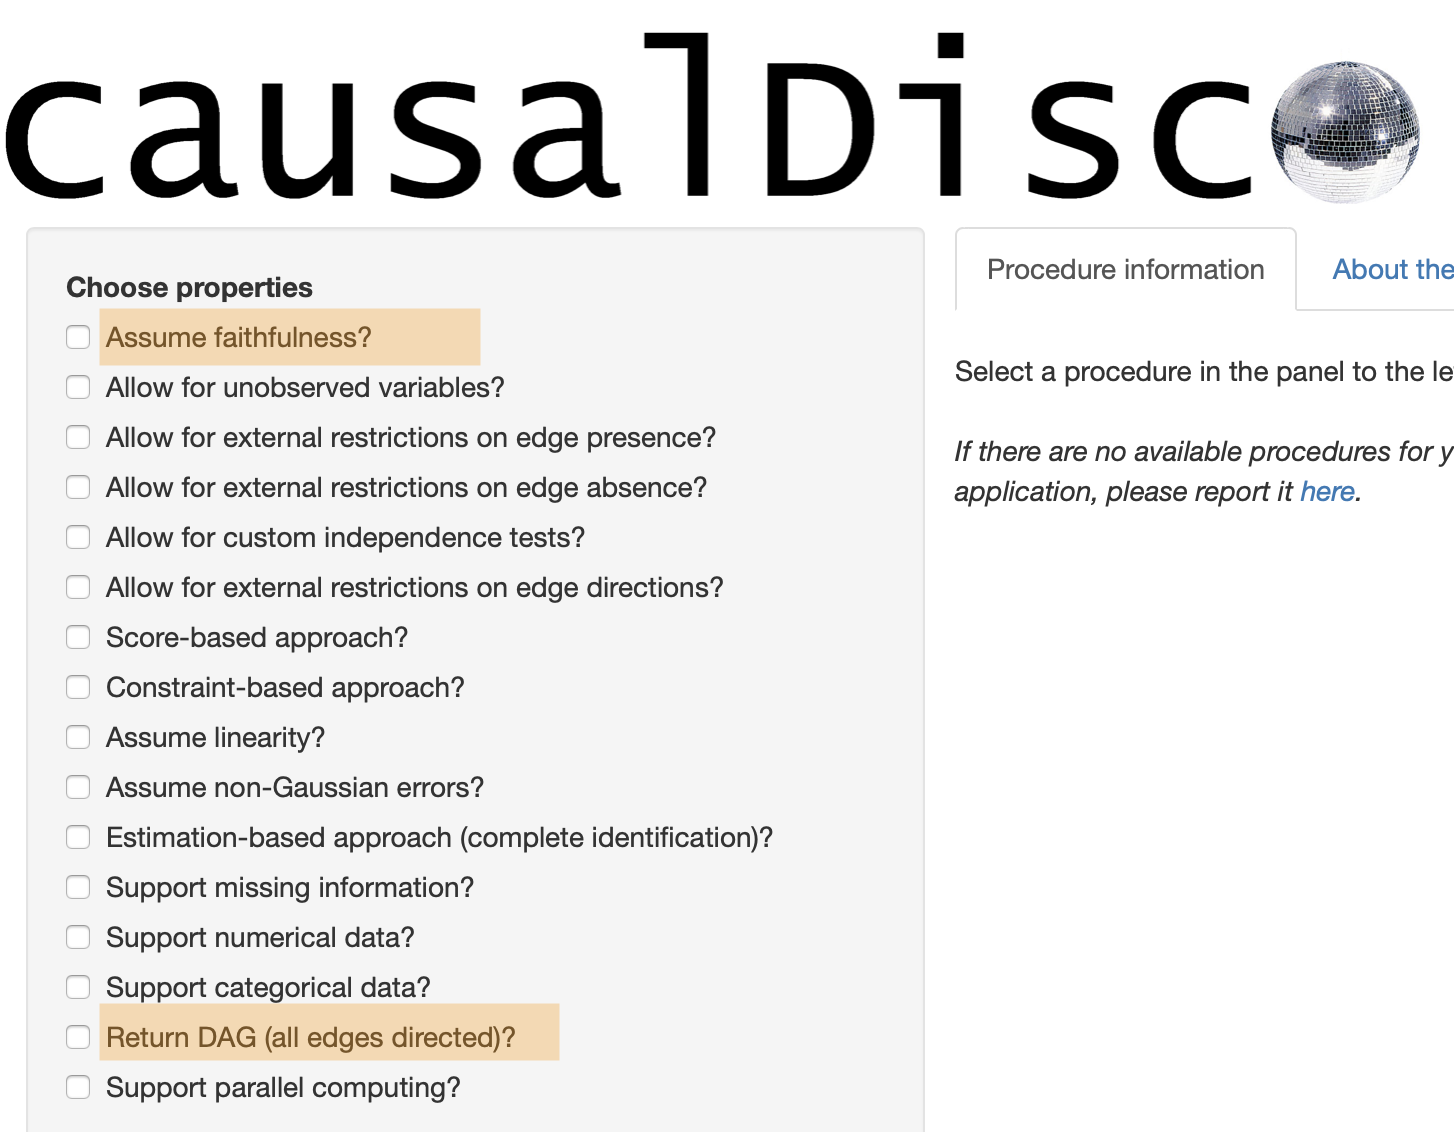
\includegraphics[scale=.4]{pics/causalDisco_marked}	
\end{frame}

\begin{frame}{Faithfulness}
	If $f$ factorizes with respect to the DAG $G$ then
	$$
	S \mbox{ d-separates }A \mbox{ and }B \mbox{ in }G \qquad\Longrightarrow\qquad A\indep B|S.
	$$
	At least in principle, $f$ may satisfy some additional conditional independence statements so the reverse implication may not hold. \\[.3cm]
	$f$ is \alert{faithful} to the DAG $G$ if 
	$$
	S \mbox{ d-separates }A \mbox{ and }B \mbox{ in }G \qquad\Longleftrightarrow\qquad A\indep B|S.
	$$
	\smallskip 
	
	This assumption is not entirely innocent:\\
	{\scriptsize Uhler, C., Raskutti, G., B\"{u}hlmann, P., \& Yu, B. (2013). Geometry of the faithfulness assumption in causal inference. The Annals of Statistics.}
\end{frame}

\begin{frame}{PC algorithm}
Currently one of the most popular algorithms.
	\begin{alertblock}{Stage one: Learn the skeleton.}
Use the fact that \qquad $u\not\sim v\quad\Longleftrightarrow\quad \exists S\subseteq V\mbox{ s.t. }u\indep v|S$.\\[.2cm]
 {\small Starting with the complete graph, conditional independences with an increasing order are tested and edges are removed.}
\end{alertblock}
	\begin{alertblock}{Stage two: Learn the edge directions.}
Several algorithms are implemented in \texttt{pcalg}
\end{alertblock}
\end{frame}

\begin{frame}[fragile]{Application for CAD data}
Load the data and learn the CP tables.	\begin{lstlisting}
library(pcalg); library(gRbase)
# use again the CAD dataset. coding {0,1} and {0,1,2}
cad <- data.matrix(cad1)-1; 
# 236 observations on 14 variables (one ternary, 13 binary)
 \end{lstlisting}
Run the PC algorithm with the implemented discrete independence test.
	\begin{lstlisting}
suffStat <- list(dm=cad,nlev=rep(2,14)+diag(14)[2,],adaptDF=TRUE)
cad.bn <- pc(suffStat,disCItest,alpha=0.1,labels=colnames(cad))
qgraph::qgraph(cad.bn)
 \end{lstlisting}
The package has also implemented testing CI for binary distributions (function \texttt{binCItest}) and also any external function can be called here.
\begin{itemize}
	\item may be important in case of small sample sizes as in the example above.
\end{itemize}
\end{frame}

\begin{frame}{}
	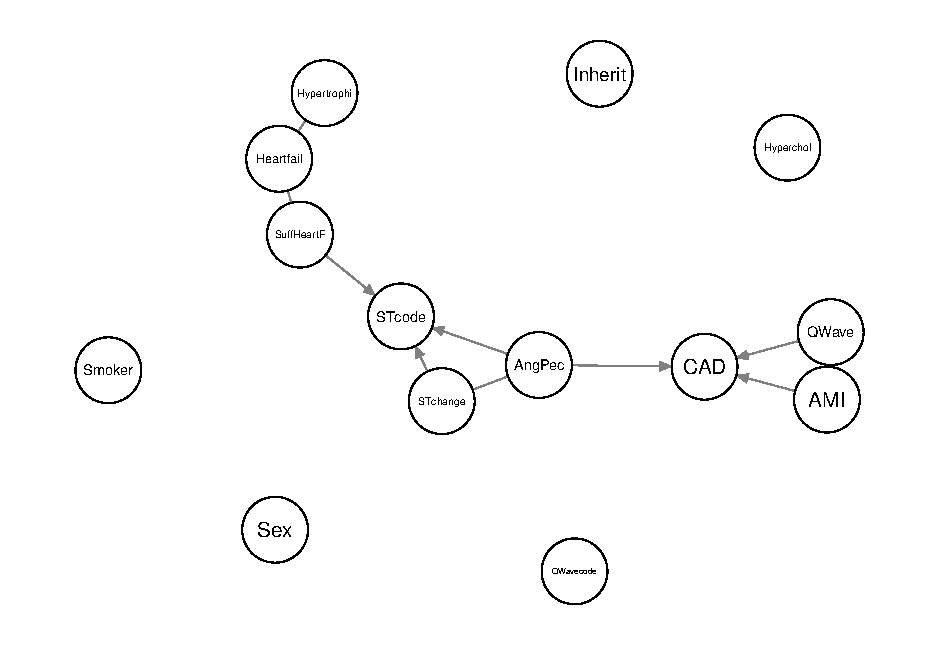
\includegraphics[width=\textwidth]{pics/CAD_PC}
\end{frame}

\begin{frame}[fragile]{}
We use part of the CAD data to obtain a data set of binary variables.
	\begin{lstlisting}
# remove the ternary variable
cad2 <- data.matrix(cad1[,-2])-1; 
# 236 observations on 13 binary variables
suffStat <- list(dm=cad2,adaptDF=TRUE)
# m.max=4 because otherwise the estimates unreliable
cad.bn <- pc(suffStat,binCItest,alpha=0.1,labels=colnames(cad2),m.max=4)
qgraph::qgraph(cad.bn)
 \end{lstlisting}
 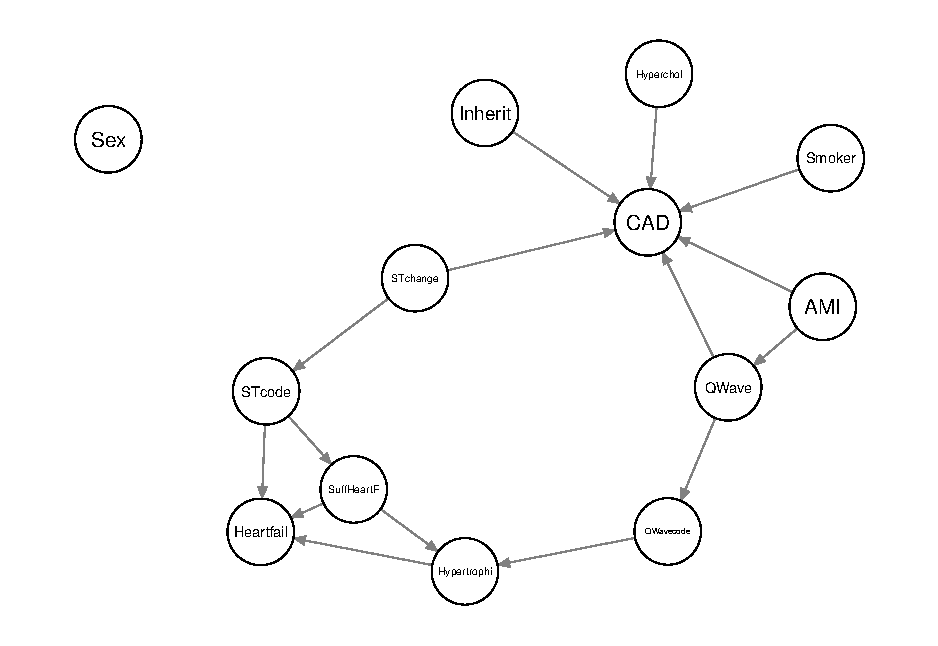
\includegraphics[scale=.55]{pics/CAD_bin}
\end{frame}


\begin{frame}{Markov equivalence}
Only very rarely we can identify the underlying DAG from \textcolor{blue}{observational data}.\\[.2cm] 
\begin{beamercolorbox}[wd=\paperwidth,sep=5pt]{important}
	DAGs can be learned only up to some equivalence class.
\end{beamercolorbox}
\smallskip 
	e.g.\quad $\overset{1}{\bullet}\to \overset{2}{\bullet}$, $\overset{1}{\bullet}\leftarrow \overset{2}{\bullet}$, and $\overset{1}{\bullet}- \overset{2}{\bullet}$ all define the same model.\\[.2cm]
	
\begin{beamercolorbox}[wd=\paperwidth,sep=5pt]{result}	Two DAGs are \textbf{Markov equivalent} (define the same statistical model) if and only if they have the same skeleton and v-structures.
\begin{itemize}
	\item \alert{Essential graph} describes the Markov equivalence class. 
\end{itemize}
\end{beamercolorbox} 
\medskip
\begin{beamercolorbox}[wd=\paperwidth,sep=5pt]{important}
	In certain scenarios there is a way around this, which we will discuss:
	\begin{itemize}
		\item Use interventions (experimental economics?)
		\item Instead of a DAG, assume an underlying Structural Causal Model.
		\item Anchors and invariance. (not discussed here)
	\end{itemize}
\end{beamercolorbox}
\end{frame}

\begin{frame}[fragile]{Visualize the essential graph}
\begin{lstlisting}
library(ggm)
qgraph::qgraph(as(essentialGraph(amat(chestdag)),"graphNEL"))
\end{lstlisting}
\begin{center}
	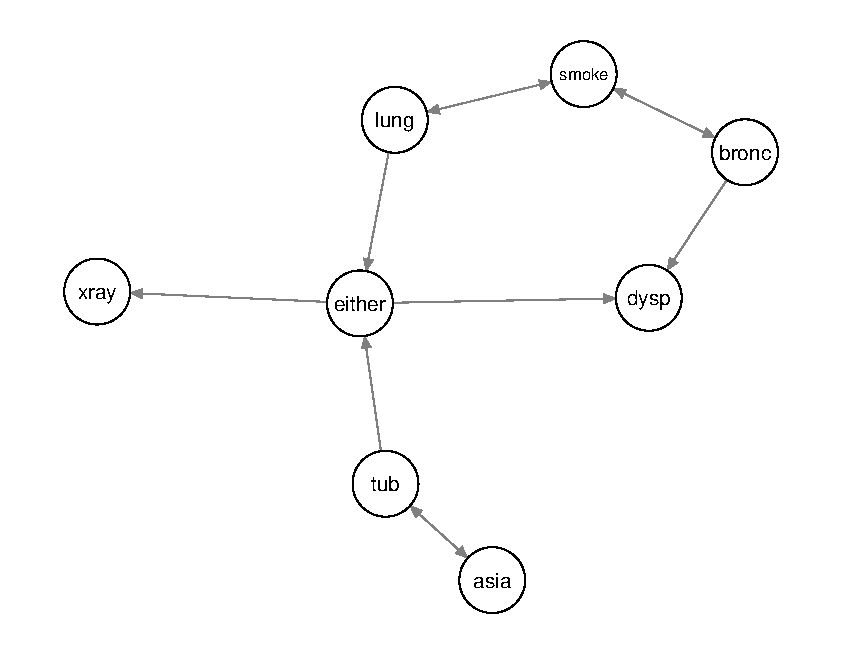
\includegraphics[scale=.6]{pics/chestdag_equiv}
\end{center}
\end{frame}

\subsection{Structural causal models}

\begin{frame}[plain,noframenumbering]{}
\begin{center}
	{\huge \textcolor{DarkRed}{4.2 Structural Causal Models}}
\end{center}
\end{frame}

\begin{frame}[fragile,label=SCM]{Structural Causal Models}
	A structural causal model (SCM) consists of a collection of $m$ structural assignments
	$$
	X_i\;:=\;f_i(\pa_i,\epsilon_i)\qquad\mbox{for }i=1,\ldots,m,
	$$
	where $\pa_i\subset \{X_1,\ldots,X_m\}\setminus \{X_i\}$ and all $\epsilon_i$ are independent of each other. \\[.2cm]
	The underlying graph $G$ of an SCM is defined in the obvious way.
	\begin{alertblock}{If $G$ is a DAG, sampling data from SCMs is easy}
		Sample from the SCM: $X_1=X_3^2+\epsilon_1$, $X_2=\sin(X_3)+\epsilon_2$, $X_3=\epsilon_3$, $X_4=X_2+e^{X_3+\epsilon_4}$, with $\epsilon_i$ having respectively normal, chi-squared, uniform, and normal distribution.  
		\begin{lstlisting}
set.seed(1); n <- 100
X3 <- runif(n)-0.5
X1 <- X3*X3 +rnorm(n)
X2 <- sin(X1)+rnorm(n)^2
X4 <- X2+exp(X3+rnorm(n))
X <- cbind(X1,X2,X3,X4)
\end{lstlisting}
	\end{alertblock}
\end{frame}

\begin{frame}[fragile]{Gaussian DAG models}
\begin{alertblock}{Linear Structural Equation models}
	Let $\varepsilon_1, \ldots,\varepsilon_m$ be independent variables. Consider a model
		$$
		X_i \;=\;\sum_{j\in {\rm pa}(i)}\lambda_{ij}X_j\;+\;\varepsilon_i.
		$$
\end{alertblock}
\begin{beamercolorbox}[wd=\paperwidth,sep=2pt]{important}
The \textcolor{SeaGreen}{Gaussian DAG models} are precisely the Linear Structural Equation models on DAGs, where $\epsilon_i$ are independent Gaussian variables.
\end{beamercolorbox} 
The function \texttt{fitDag} in the \textbf{ggm} package fits Gaussian DAGs.
	\begin{lstlisting}
> library(ggm); data(carcass); S.carc <- cov(carcass)
> gdag1 <- DAG(LeanMeat~Meat13:Fat11:Fat12, Meat13~Meat11:Meat12,Fat12~Fat11,Fat13~Meat11:Meat12,Meat12~Meat11)
> qgraph::qgraph(as(gdag1,"graphNEL"))  # to visualize the DAG
> fdag1 <- fitDag(gdag1, S.carc,nrow(carcass))
> fdag1$dev # the deviance is really large and the p-value is basically 0.
[1] 552.2726\end{lstlisting}
\end{frame}

\begin{frame}[fragile]{Interventions}
Recall: Typically impossible to identify the DAG from observational data. 	\\[.3cm]
Things are better if we can observe the system under \alert{intervention} or  include the domain knowledge.\\[.3cm]
We consider only the simplest way to intervene by fixing a value of a variable. 

\medskip
Consider the example on Slide~\ref{SCM} with $X_2 \leftarrow 1$
\begin{lstlisting}
set.seed(1); n <- 100
X3 <- runif(n)-0.5
X1 <- X3*X3 + rnorm(n)
X2 <- 1
X4 <- X2+exp(X3+rnorm(n))
X <- cbind(X1,X2,X4)
\end{lstlisting}

The distribution of $(X_1,X_3)$ did not change!
\end{frame}

\begin{frame}[fragile]{}
\begin{lstlisting}
scm = model2network("[X3][X1|X3][X2|X1][X4|X2:X3]")
bnlearn::dsep(scm, "X2", "X3","X1")	
qgraph::qgraph(essentialGraph(amat(scm)))
\end{lstlisting}
There are two DAGs Markov equivalent to the DAG of this SCM.
\begin{center}
	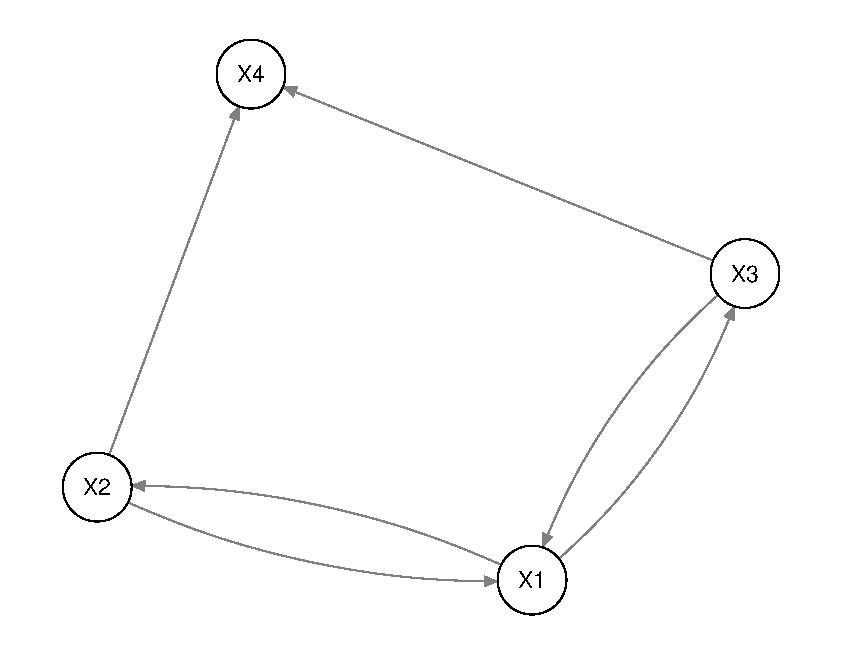
\includegraphics[scale=.4]{pics/scm_essential}
\end{center} 
In one of them the distribution of $X_1$ under $X_2\leftarrow 1$ changes. Intervening on $X_3$ allows us to pin down the original DAG. 
\end{frame}

%\begin{frame}{Topics we omit	}
%	Many different types of graphical models are used.
%	\begin{enumerate}
%		\item undirected graphical models (aka Markov random fields)
%		\item models of DAGs (aka Bayesian Networks)
%		\item chain graph models
%		\item mixed graph models
%		\item  
%	\end{enumerate}
%\end{frame}

%\subsection{Causality}

%\begin{frame}[plain,noframenumbering]{}
%\begin{center}
%	{\Huge \textcolor{DarkRed}{4. Causality}}
%\end{center}
%\end{frame}
%
%\begin{frame}{Association versus causation}
%	gg
%\end{frame}

\begin{frame}{More on learning the DAG}
\begin{beamercolorbox}[wd=\paperwidth,sep=5pt]{important}
If $X$ is induced by a Structural Causal Model with graph $G$ then $X$ satisfies the Markov properties with respect to $G$. The model is often strictly smaller	than the underlying DAG model, which allows for graph identification. 
\end{beamercolorbox}
\bigskip

Some cases when identification is possible:
\begin{itemize}
	\item In linear models if $\varepsilon$ are non-Gaussian, the DAG can be recovered. Linear non-Gaussian acyclic model (\alert{LiNGAM}).
	\item Additive noise models: $X_i=f_i(X_{\pa(i)})+\epsilon_i$ with nonlinear $f_i$, Gaussian $\epsilon_i$. 
\end{itemize}
\end{frame}

\begin{frame}[fragile]{LiNGAM in action}
	Package \texttt{CompareCausalNetworks} provides a unified interface for the estimation of causal networks that includes a handful of available methods (also LiNGAM).\\[.3cm]
		\begin{lstlisting}
library(CompareCausalNetworks)
# use again the CAD dataset. remove one non-binary variable
data(cad1,package='gRbase')
cad <- data.matrix(cad1)-1; 
g.cad <- getParents(cad, method="LINGAM") # learn the DAG
qgraph::qgraph(g.cad)
 \end{lstlisting}

\end{frame}

%\end{document}

\section{GMs with latent variables}

\begin{frame}[plain,noframenumbering]{}
\begin{center}
	{\Huge \textcolor{DarkRed}{5. GMs with latent variables}}
\end{center}
\end{frame}

%\begin{frame}{Idea}
%	Partial correlations allow to measure association between random variables with the effect of potentially confounding variables removed. \\
%	However, if the confounding variables are unobserved, or are simply not included the data set, this will not work. 
%\end{frame}

\begin{frame}{What is a hidden variable?}
	Random vector $Y=(X,H)$: $X$ observed, $H$ \alert{hidden/latent}. \\[.3cm]
	Observing $X$, we only get information about the marginal $p_X$.\\[.3cm]
	Since $p(x)=\sum_h p(h)p(x|h)$, sometimes $p(x)$ may be enough to recover $p(x,h)$.
	\begin{exampleblock}{Examples}
		Factor analysis models, hidden Markov models, Markov switching models, mixture models.
	\end{exampleblock}
		\begin{exampleblock}{Further Examples}
		Latent tree models, ancestral graph models, nested Markov models.
	\end{exampleblock}

\end{frame}


\begin{frame}{Simpson's paradox}
%	Two real-valued random variables  $X$ and $Y$ are \alert{positively associated} if ${\rm cov}\{f(X),g(Y)\}\geq 0$ for all $f$, $g$ which are non-decreasing.

%\pause

\alert{The Yule-Simpson paradox} says that we may have $X$ and $Y$ positively associated but $X$ and $Y$ negatively associated conditionally on a third variable $Z$. \\[.3cm]
\begin{center}
	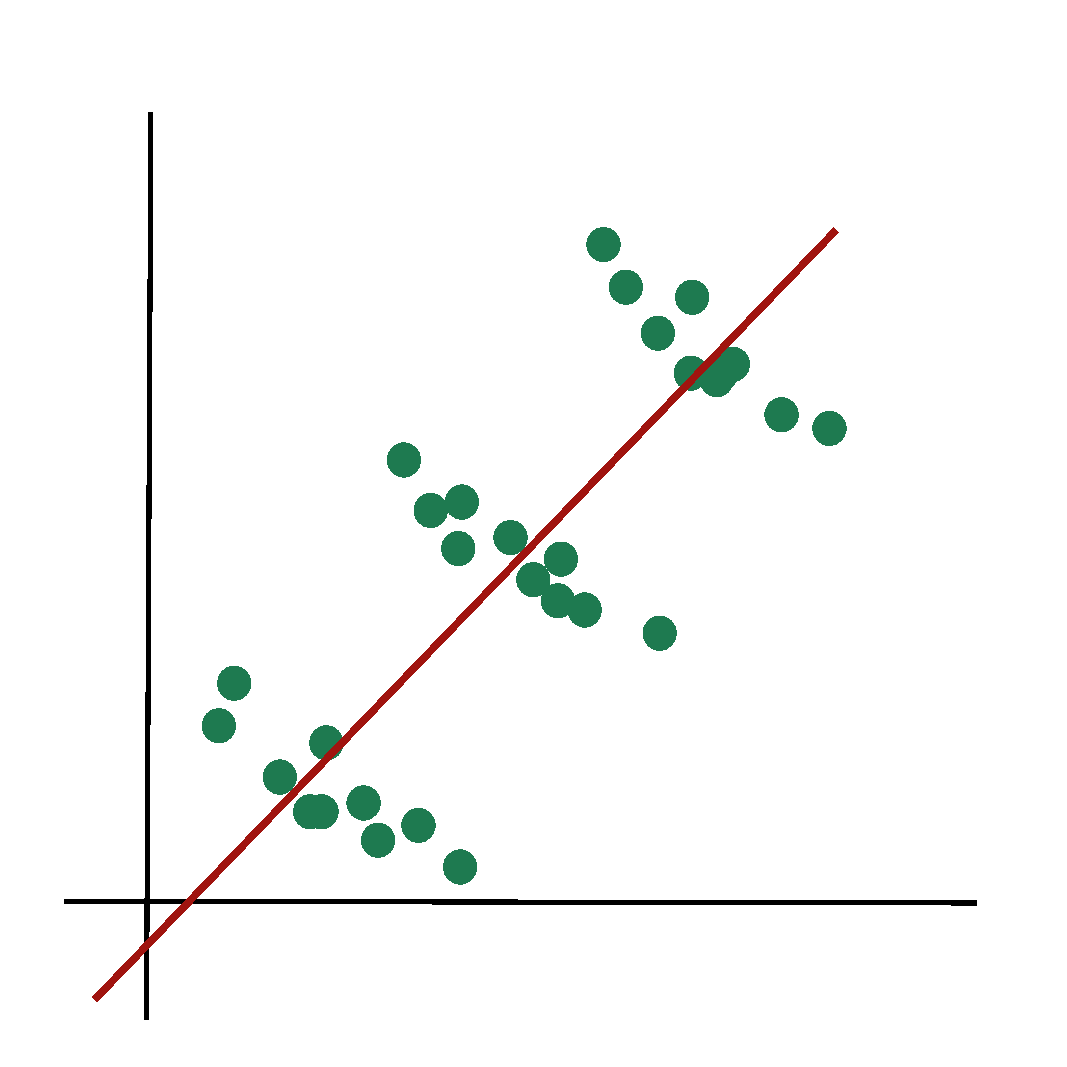
\includegraphics[scale=.2]{pics/simpson}
\end{center}
This together with two examples discusses in Part I shows how important is to observe all variables relevant for the causal analysis. \\[.2cm]
Often there is a way to tell that such a missing variable exists.
\end{frame}

\begin{frame}{Fixed graph}
	If the graph is fixed then, at least in principle, estimation can be performed using the \alert{EM algorithm} (usual disadvantages).\\[.5cm]
	If the  graph is decomposable, the M-step is given in closed form.
	\begin{itemize}
		\item packages discussed earlier will apply.\\[.5cm]
	\end{itemize}
	An example of the E-step for the Gaussian case appears on the next slide.\\[.5cm]
%	A typical example is the latent class model or the factor analysis model. Several R packages are available. 
%%	\begin{lstlisting}
%		library(poLCA)
%	\end{lstlisting}
\end{frame}

\begin{frame}[label=Estep]{The $E$-step for Gaussian distributions}
\begin{itemize}
\item The $E$-step is standard. We work with data of length $n$ normalized to have mean zero.  
\item Suppose that $\Sigma$ represents the \textbf{full} covariance matrix estimated at the previous step of the algorithm.
\item Let $S$ be the sample correlation matrix that we are trying to estimate: 
$S_{XX}=\frac{1}{n} \bs X^T \bs X,\quad S_{HX}=\frac{1}{n} \bs H^T \bs X,\quad S_{HH}=\frac{1}{n} \bs H^T \bs H$,
\item Standard formulas: $\E[H|X]\quad =\quad \Sigma_{HX}\Sigma_{XX}^{-1}X$ and ${\rm var}(H|X)=\Sigma_{HH}-\Sigma_{HX}\Sigma_{XX}^{-1}\Sigma_{XH}$.
\item This gives $\E[S_{HX}|\bs X]\quad =\quad \Sigma_{HX}\Sigma_{XX}^{-1}S_{XX}$
and
$$\E[S_{HH}|\bs X]=\Sigma_{HH}-\Sigma_{HX}\Sigma_{XX}^{-1}\Sigma_{XH}+\Sigma_{HX}\Sigma_{XX}^{-1}S_{XX}\Sigma_{XX}^{-1}\Sigma_{XH}.$$
\end{itemize}
\end{frame}


\begin{frame}{Learning the graph structure}
Learning the graph structure in the presence of latent variables is hard:
\begin{itemize}
	\item The number of possible graphs is too large (in fact infinite).
	\item Estimation for each fixed graph is relatively complicated.
	\item Models with latent variables fail many regularity assumptions used in standard asymptotic statistics.
\end{itemize}
\bigskip

Some \texttt{R} packages: \texttt{lvnet}, \texttt{pcalg} (method \texttt{FCI}), \texttt{HMM}. 
\begin{alertblock}{Some cases we cover:}
\begin{itemize}
	\item Latent tree models.
	\item Latent Gaussian graphical models in high dimensions.
	\item Briefly: \texttt{FCI} for ancestral graphs.
\end{itemize}
\end{alertblock}
\end{frame}

\subsection{Latent tree models}

\begin{frame}[plain,noframenumbering]{}
\begin{center}
	{\huge \textcolor{DarkRed}{5.1 Latent tree models}}
\end{center}
\end{frame}


\begin{frame}{Trees}
\begin{itemize}
\item \textbf{Definition}: \textcolor{blue}{Tree} $=$ undirected graph without cycles\\[.3cm]
\item a tree $T=(V,E)$: $V$ \textcolor{blue}{vertices},\quad $E$ \textcolor{blue}{edges}\\[.4cm]
\begin{minipage}{4cm}
\begin{center}
\tikzstyle{vertex}=[circle,fill=black,minimum size=5pt,inner sep=0pt]
\tikzstyle{hidden}=[circle,draw,minimum size=5pt,inner sep=0pt]
  \begin{tikzpicture}[scale=.7]
  \node[hidden] (1) at (-.7,.7)   {};
    \node[hidden] (2) at (-.7,-.7) {};
    \node[hidden] (3) at (1.1,.9) {};
    \node[hidden] (4) at (2.2,.9) {};
    \node[hidden] (5) at (4,0.7) {};
    \node[hidden] (6) at (4,-.7) {};
    \node[hidden] (a) at (0,0) {};
    \node[hidden] (b) at (1.1,0) {};
    \node[hidden] (c) at (2.2,0) {};
     \node[hidden] (d) at (3.3,0) {};
     \draw[line width=.3mm] (a) to (1);
    \draw[line width=.3mm] (a) to (2);
    \draw[line width=.3mm] (a) to (b);
    \draw[line width=.3mm] (b) to (3);
    \draw[line width=.3mm] (b) to (c);
    \draw[line width=.3mm] (c) to (4);
   \draw[line width=.3mm] (d) to (c);
   \draw[line width=.3mm] (d) to (5);
   \draw[line width=.3mm] (d) to (6);
  \end{tikzpicture}\\
  undirected
  \end{center}
\end{minipage}\hspace{1cm}
\begin{minipage}{4cm}
\begin{center}
\tikzstyle{vertex}=[circle,fill=black,minimum size=5pt,inner sep=0pt]
\tikzstyle{hidden}=[circle,draw,minimum size=5pt,inner sep=0pt]
  \begin{tikzpicture}[scale=.7]
  \node[hidden] (1) at (-.7,.7)   {};
    \node[hidden] (2) at (-.7,-.7) {};
    \node[hidden] (3) at (1.1,.9) {};
    \node[hidden] (4) at (2.2,.9) {};
    \node[hidden] (5) at (4,0.7) {};
    \node[hidden] (6) at (4,-.7) {};
    \node[hidden] (a) at (0,0) [label=above:$r$]{};
    \node[hidden] (b) at (1.1,0) {};
    \node[hidden] (c) at (2.2,0) {};
     \node[hidden] (d) at (3.3,0) {};
     \draw[->,-latex,line width=.3mm] (a) to (1);
    \draw[->,-latex,line width=.3mm] (a) to (2);
    \draw[->,-latex,line width=.3mm] (a) to (b);
    \draw[->,-latex,line width=.3mm] (b) to (3);
    \draw[->,-latex,line width=.3mm] (b) to (c);
    \draw[->,-latex,line width=.3mm] (c) to (4);
   \draw[->,-latex,line width=.3mm] (c) to (d);
   \draw[->,-latex,line width=.3mm] (d) to (5);
   \draw[->,-latex,line width=.3mm] (d) to (6);
  \end{tikzpicture}\\
  \textcolor{blue}{rooted}
  \end{center}
\end{minipage}
\end{itemize}
\vspace{.5cm}
\begin{minipage}{6cm}
\begin{itemize}
\item rooted tree often depicted as\ldots\\[.3cm]
\item \textcolor{blue}{leaves}=degree one nodes\\[.3cm]
\item \textcolor{blue}{inner nodes}=degree $\geq 2$ nodes
\end{itemize}
\end{minipage}
\begin{minipage}{4cm}
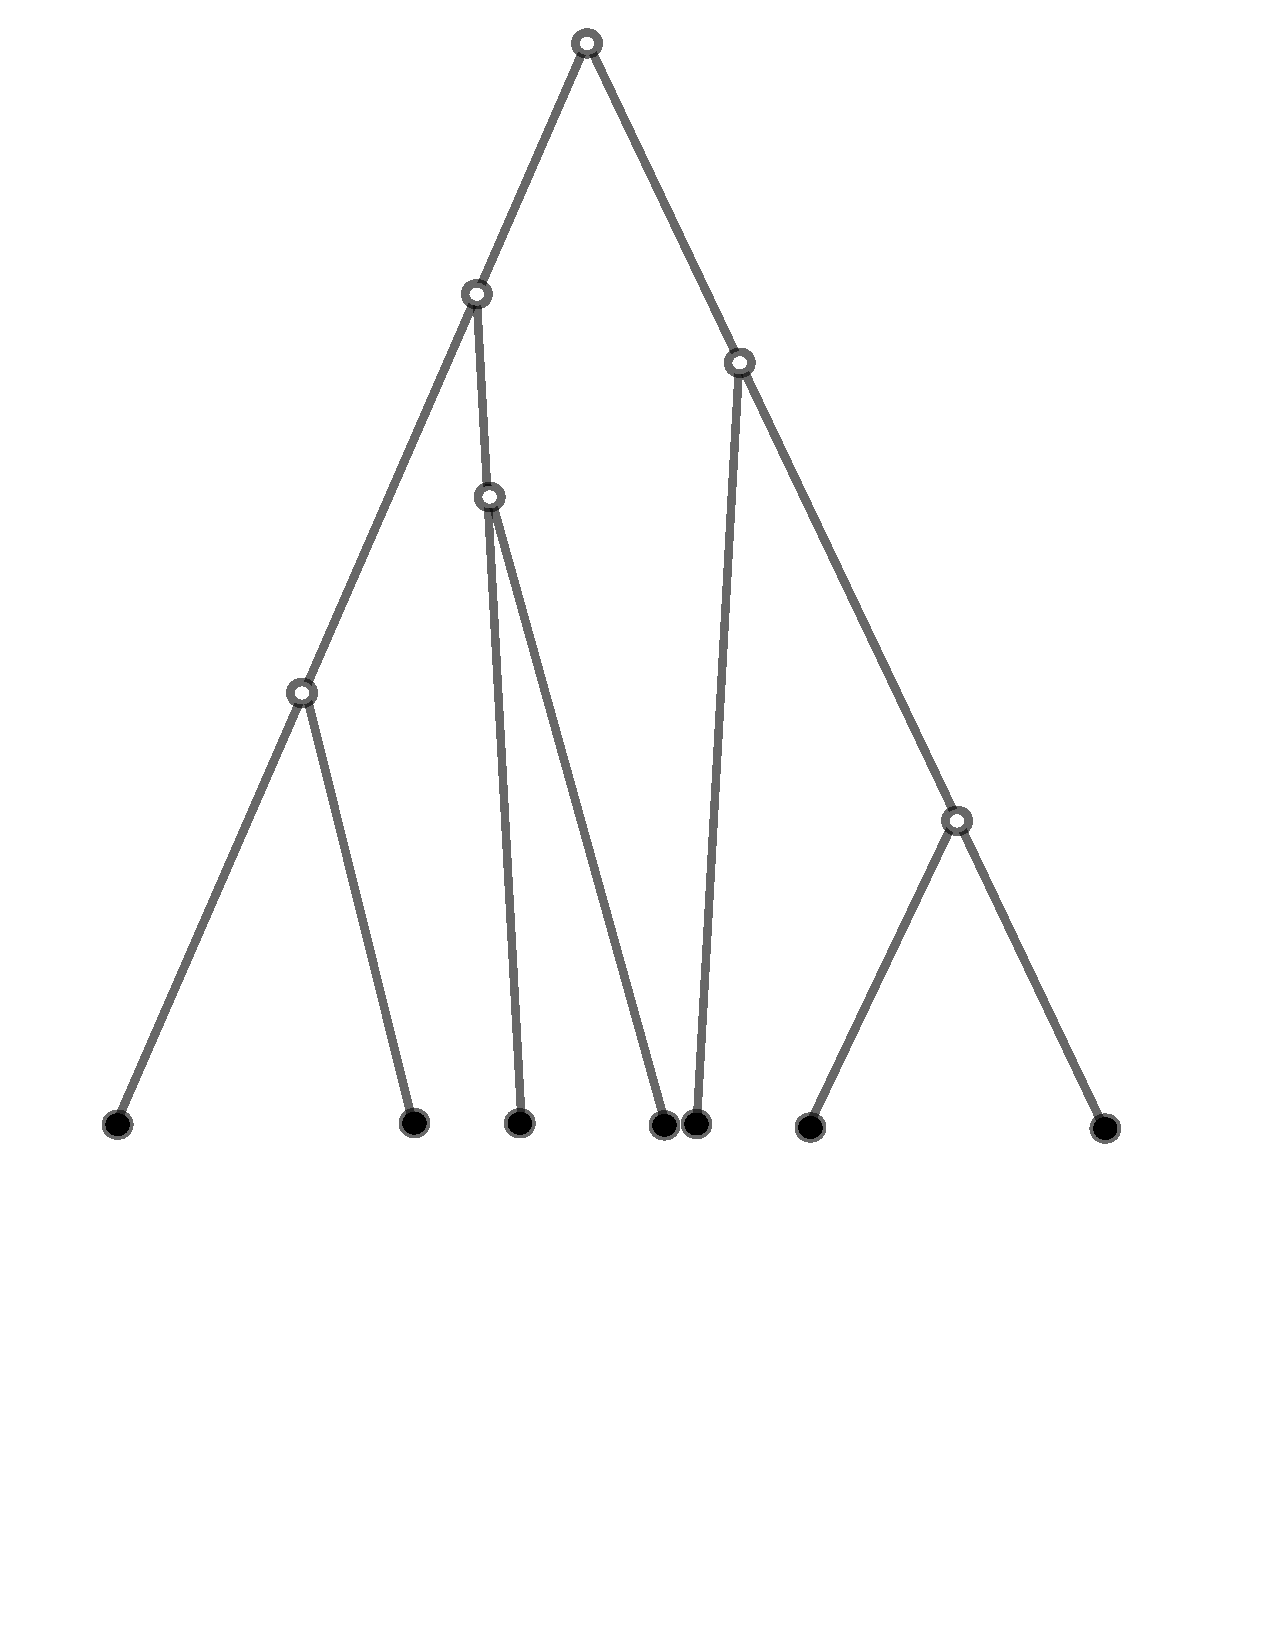
\includegraphics[scale=.15]{./pics/rtree}
\end{minipage}
\end{frame}



\begin{frame}{Latent tree models}
		\begin{alertblock}{One step away from tree models}
\begin{itemize}
\item Graphical models on trees have many nice properties: 
\begin{itemize}
\item exponential families with explicit formulas for the MLE,
\item dynamic programming for efficient computations of various probabilistic quantities.
\end{itemize}
\item Making some of the variables hidden gives greater flexibility.\end{itemize}
	\end{alertblock}
	\begin{alertblock}{Naive definition of latent tree models}
\begin{itemize}
\item \textcolor{blue}{Tree-decomposable distribution} a marginal distribution of a tree distribution.
\item Discussed by J. Pearl as a natural extension of star-decomposable distributions (mixture model, naive Bayes model, latent class model)
\end{itemize}
	\end{alertblock}
	{\tiny Judea Pearl, \textit{Fusion, Propagation, and Structuring in Belief Networks}, Artificial Inteligence, 1986.
	}
\end{frame}


\begin{frame}{Motivation}
	\begin{alertblock}{Statistical motivation}
	\begin{itemize}
	\item Applications in: 
	\begin{itemize}
	\item phylogenetics and linguistics -- to model evolutionary processes,
	\item hierarchical clustering,
	\item image processing and network tomography.
	\end{itemize}
	\item Important concept in causality.
	\item Many well known statistical models are submodels:
	\begin{itemize}
	\item hidden Markov models and naive Bayes models,
	\item phylogenetic models of evolution.
	\end{itemize}
	\end{itemize}
	\end{alertblock}
%	\vspace{-.3cm}
%\begin{alertblock}{Mathematical motivation}
%\begin{itemize}
%\item Understand models with hidden data:
%\begin{itemize}
%\item identifiability, model constraints, 
%\item geometry of the likelihood function.
%\end{itemize}
%\end{itemize}
%\end{alertblock}
%	{\tiny 	Alan S. Willsky, \textit{Multiresolution Markov Models for Signal and Image Processing}, 2002.\\
%	Martin J. Wainwright, Michael I. Jordan, \textit{Graphical Models, Exponential Families, and Variational Inference}, 2008.\\
%	}
%
\end{frame}

%\begin{frame}{}
%	\begin{alertblock}{Four main statistical problems:}
%\begin{itemize}
%\item Learn the underlying tree.
%\item Learn the underlying parameter $\theta$.
%\item Given an estimator $\hat \theta$, compute various marginal probabilities from (the fully observed distribution) $p(y;T,\hat \theta)$.
%\item Test the tree model hypothesis.
%\end{itemize}
%	\end{alertblock}
%\begin{beamercolorbox}[wd=\paperwidth,sep=5pt]{goldbox}
%	Depending on the application, some problems are irrelevant.
%\end{beamercolorbox}
%\end{frame}



\begin{frame}{Gaussian latent tree model}
\begin{itemize}
%\item The latent tree Gaussian model is denoted by $M(T)$.
\item If $Y=(X,H)$ is jointly Gaussian, then the marginal distribution of $X$ is also Gaussian and it satisfies
$$
\rho_{ij}=\prod_{e\in \overline{ij}} \rho_{e}\quad\mbox{for all }i,j\in [m],
$$
where $\rho_{e}$ are edge correlations. 
\item Moreover, variances $\sigma_{ii}$ for $i\in [m]$ are unconstrained.
\end{itemize}
%\vspace{.5cm}
%\begin{beamercolorbox}[wd=\paperwidth,sep=5pt]{notabene}	
%The variances of unlabeled nodes do not appear in the parametrization and so they are assumed to be equal to $1$.
%\end{beamercolorbox}
\end{frame}

\begin{frame}{Featured on my website}
\begin{beamercolorbox}[wd=\paperwidth,sep=5pt]{result}	
		\begin{minipage}{2.2cm}
	\tikzstyle{vertex}=[circle,fill=black,minimum size=5pt,inner sep=0pt]
\tikzstyle{hidden}=[circle,draw,minimum size=5pt,inner sep=0pt]
  \begin{tikzpicture}[scale=.7]
  \node[vertex] (1) at (-.8,.6)  [label=above:$1$] {};
    \node[vertex] (2) at (.8,.6) [label=above:$2$]{};
    \node[vertex] (3) at (0,-.9)  [label=below:$3$] {};
    \node[hidden] (a) at (0,0) {};
    \draw (a) to (1);
    \draw (a) to (2);
    \draw (a) to (3);
  \end{tikzpicture}
	\end{minipage}
\begin{minipage}{5cm}
\begin{itemize}
\item Consider the tripod tree model. 
\item $Y=(X_{1},X_{2},X_{3},H)$
\item $Y\sim\mathcal N_{4}(0,\Sigma)$, $\Sigma\in  N(T)$\end{itemize}
\end{minipage}
\end{beamercolorbox}
\begin{itemize}
\item $\rho_{12}=\rho_{h1}\rho_{h2}$, $\rho_{13}=\rho_{h1}\rho_{h3}$, $\rho_{23}=\rho_{h2}\rho_{h3}$ and $\rho_{h1},\rho_{h2},\rho_{h3}\in [-1,1]$.
\end{itemize}
\begin{center}
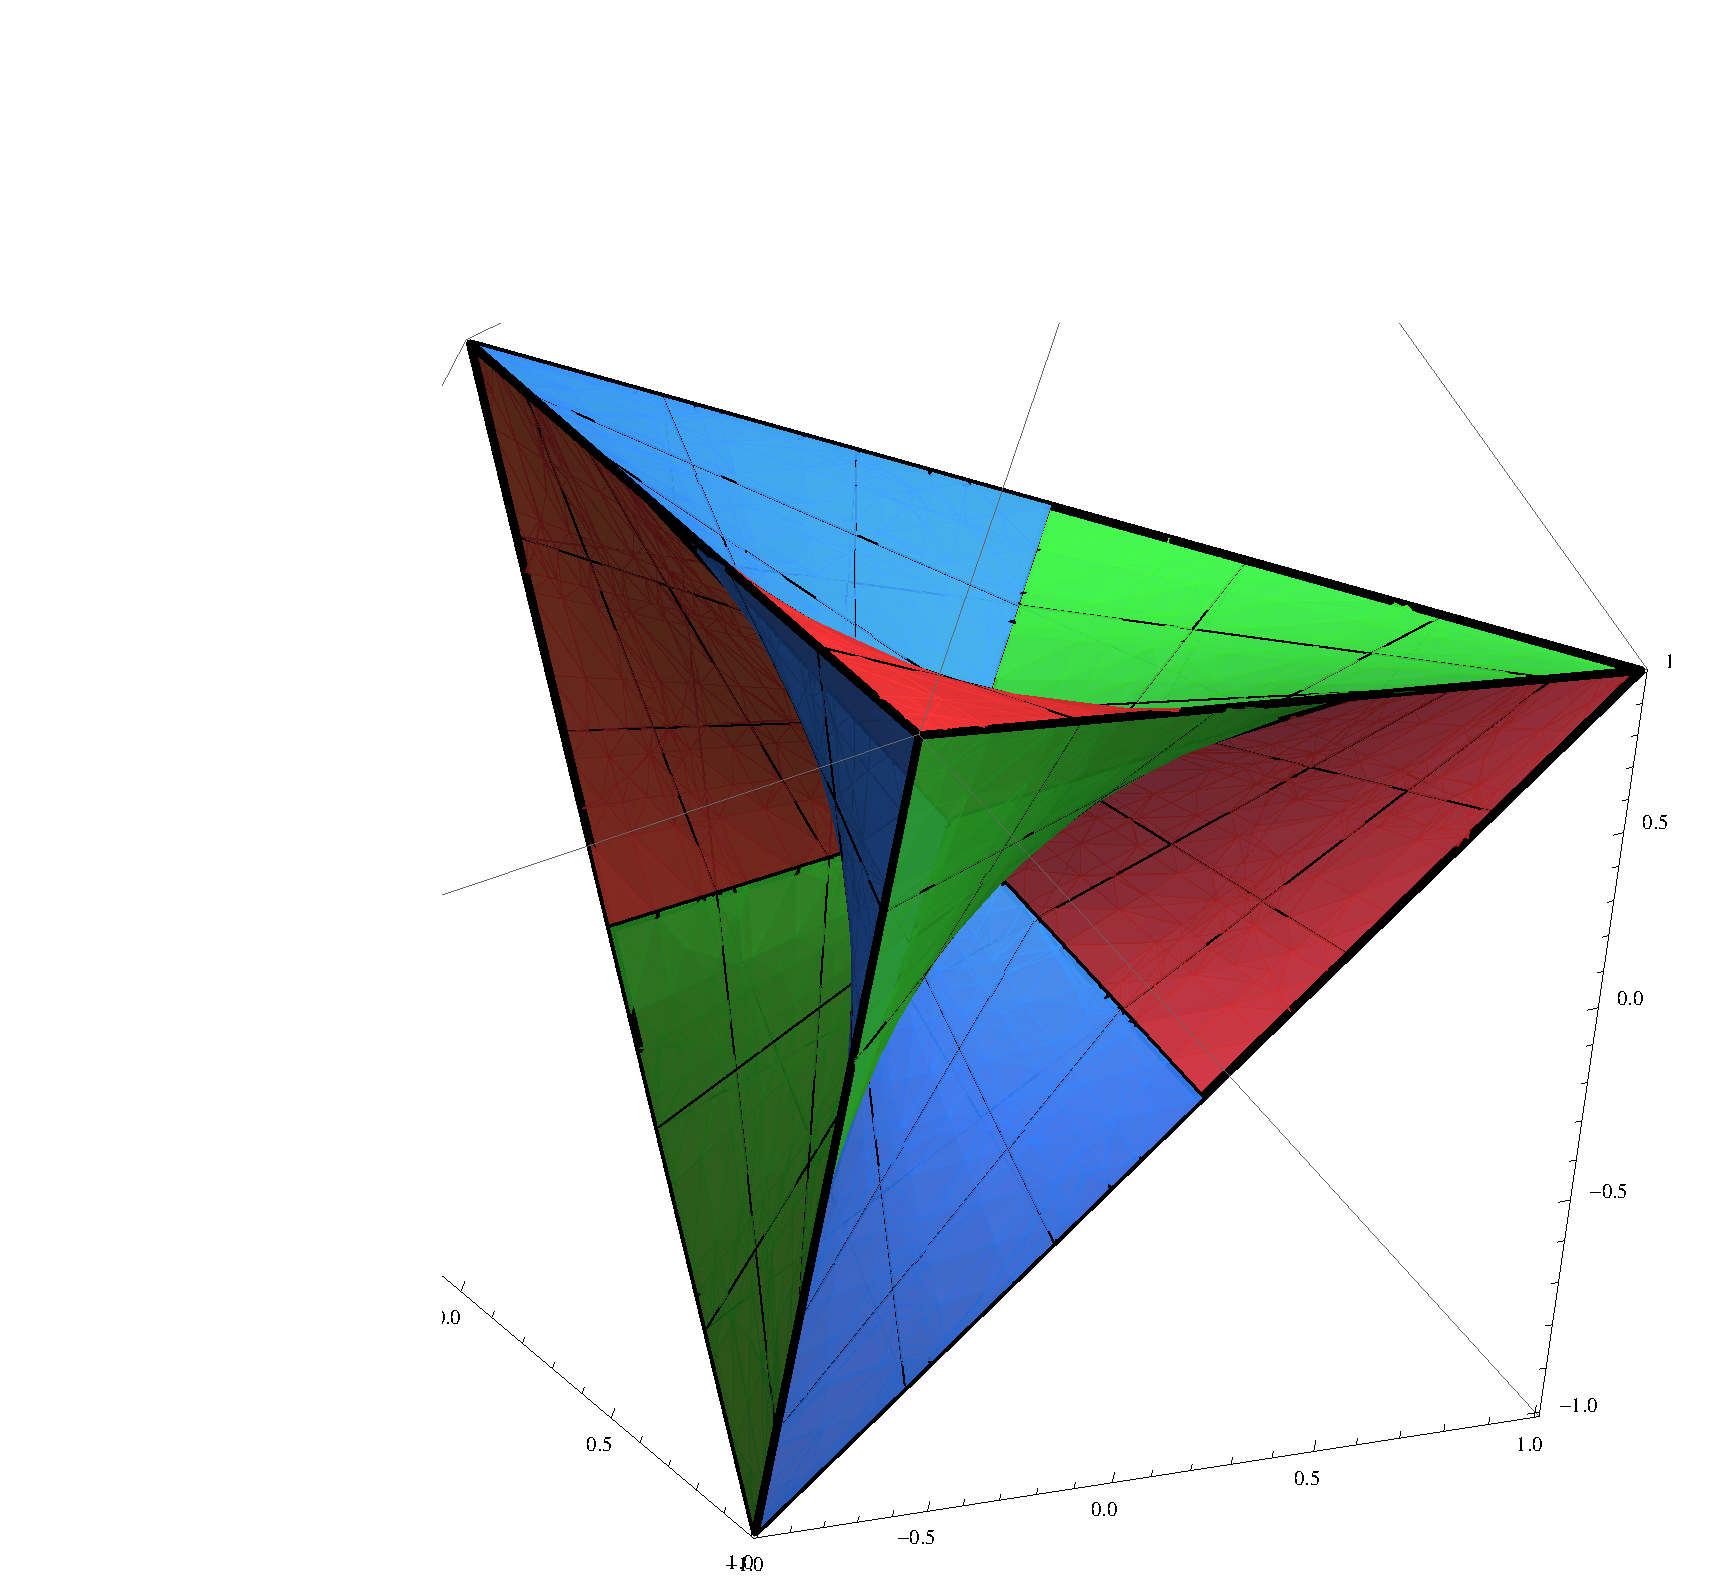
\includegraphics[scale=.21]{./pics/tripod_cut}	
\end{center}
\end{frame}

\begin{frame}
	\frametitle{Chow-Liu algorithm}
Suppose first we observe all the data. (no hidden variables)\\[.3cm]
\textbf{Problem}: Suppose that we want to find the MLE over the set of \textbf{all} tree models for this data.\\[.3cm]

\begin{beamercolorbox}[wd=\paperwidth,sep=5pt]{goldbox}
\textcolor{blue}{Mutual information} $I(Y_{i},Y_{j})$ as the Kullback-Leibler divergence between $p_{ij}$ and the product $p_{i}p_{j}$
$$
\bs I_{p}(Y_{i},Y_{j})\quad=\quad \sum_{y_{i},y_{j}} p_{ij}(y_{i},y_{j})\log\frac{p_{ij}(y_{i},y_{j})}{p_{i}(y_{i})p_{j}(y_{j})}.
$$
Moreover, $\bs I_{p}(Y_{i},Y_{j})\geq 0$ and is zero precisely when $Y_{i}$ and $Y_{j}$ are independent. 
\end{beamercolorbox}
\end{frame}



\begin{frame}
	\frametitle{}
For a fixed tree $T$: $$
p( y;\hat \theta) \quad=\quad \prod_{v}\hat p_{v}(y_{v})\prod_{u- v\in E(T)} \frac{\hat p_{uv}(y_{u},y_{v})}{\hat p_{u}(y_{u})\hat p_{v}(y_{v})}.
$$
The log-likelihood at $\hat \theta$ can be rewritten as
$$
n\sum_{v}\sum_{y_{v}}\hat p_{v}(y_{v})\log \hat p_{v}(y_{v})+\,\,n\!\!\!\!\!\!\sum_{u- v\in E(T)} \bs I_{\hat p}(Y_{u},Y_{v}).
$$
\begin{beamercolorbox}[wd=\paperwidth,sep=5pt]{goldbox}
	\textbf{Theorem}: The maximum likelihood tree is the \textcolor{blue}{maximum cost spanning tree} (use \textcolor{blue}{Kruskal's algorithm}).
\end{beamercolorbox}
\medskip 

\begin{beamercolorbox}[wd=\paperwidth,sep=5pt]{important}
	The same is true in the Gaussian case
\begin{itemize}
\item here also: $\bs I_{\hat f}(Y_{u},Y_{v})=-\frac{1}{2}\log(1-\hat\rho_{uv}^{2})$, $\hat\rho_{uv}=$ sample correlation
\end{itemize}
\end{beamercolorbox}
\end{frame}
\note[itemize]{\item 
}

\begin{frame}{Exercise: Star tree}
\begin{minipage}{2cm}
\tikzstyle{vertex}=[circle,fill=black,minimum size=5pt,inner sep=0pt]
\tikzstyle{hidden}=[circle,draw,minimum size=5pt,inner sep=0pt]
  \begin{tikzpicture}
  \node[vertex] (1) at (-.8,.6)  [label=above:$1$] {};
    \node[vertex] (2) at (.8,.6) [label=above:$2$]{};
    \node[vertex] (3) at (0,-.9)  [label=below:$3$] {};
    \node[vertex] (a) at (0,0) {};
    \node at (0.1,-0.2) [label=left:$4$] {};
    \draw (a) to (1);
    \draw (a) to (2);
    \draw (a) to (3);
  \end{tikzpicture}
\end{minipage}
\begin{minipage}{8cm}
\begin{itemize}
\item Fixing parameter values, $\theta_{4}(1)=0.6$ and $\theta_{i|4}$
$$
\begin{bmatrix}
0.7 & 0.3\\
0.4 & 0.6
\end{bmatrix},\quad \begin{bmatrix}
0.8 & 0.2\\
0.5 & 0.5
\end{bmatrix},\quad \begin{bmatrix}
0.6 & 0.4\\
0.4 & 0.6
\end{bmatrix}
$$
we obtain the data generating distribution.
\end{itemize}
\end{minipage}\vspace{.5cm}
\begin{itemize}
\item a simulated matrix of observed mutual informations:
$$
\begin{bmatrix}
\cdot & 0.000 & 0.003 & \textcolor{blue}{0.043} \\ 
\cdot & \cdot  & 0.004 & \textcolor{SeaGreen}{0.027} \\ 
\cdot & \cdot  & \cdot  & \textcolor{DarkRed}{0.045} \\ 
\cdot & \cdot  & \cdot  & \cdot  
\end{bmatrix}.
$$
\item  Algorithm: First add edges $\textcolor{DarkRed}{3-4}$ and $\textcolor{blue}{1-4}$. Then,  $\textcolor{SeaGreen}{2-4}$.  Since no more edges can be added without introducing cycles, we stop. 
\end{itemize}
\end{frame}

\begin{frame}[fragile]{}
	\begin{lstlisting}
# define a binary model on the tripod tree
q <- array(0,c(2,2,2,2))
p4 <- c(0.4,0.6)
p14 <- matrix(c(0.7,0.4,0.3,0.6),2,2)
p24 <- matrix(c(0.8,0.5,0.2,0.5),2,2)
p34 <- matrix(c(0.6,0.4,0.4,0.6),2,2)
for (i in 1:2){for (j in 1:2){for (k in 1:2){for (l in 1:2){
        q[i,j,k,l] <- p4[l]*p14[l,i]*p24[l,j]*p34[l,k]
      }}}}

# generate a sample from this model
n<- 200 #sample size
dat <- sample(1:16,n,replace=TRUE,c(q))
phat <- tabulate(dat)/n
dim(phat) <- c(2,2,2,2)

#compute mutual informations
MI <- matrix(0,4,4)
for (i in 1:3){
  for (j in (i+1):4){
    pi <- apply(phat,c(i),sum); pj <- apply(phat,c(j),sum)
    pij <- apply(phat,c(i,j),sum)
    MI[i,j]=sum(log(pij/outer(pi,pj))*pij)
  }}
MI
	\end{lstlisting}
\end{frame}




\begin{frame}
	\frametitle{Structural EM: basic idea}
\begin{alertblock}{The goal}
\begin{itemize}
\item We want to find the maximum likelihood estimator over the union of latent tree models. 
\item We can assume $T$ are binary phylogenetic trees.
\begin{itemize}
\item This can be further refined if needed.
\end{itemize}
\end{itemize}
\end{alertblock}
\bigskip
\begin{alertblock}{Exploiting the Chow-Liu algorithm}
\begin{itemize}
\item If we observed all vertices we could use the Chow-Liu algorithm.
\item We use the same idea as in the EM algorithm: first estimate the unobserved mutual informations, then run Chow-Liu on everything.
\end{itemize}
\end{alertblock}
\end{frame}

\begin{frame}
	\frametitle{Structural EM for Gaussian models}
\begin{beamercolorbox}[wd=\paperwidth,sep=5pt]{goldbox}
\begin{itemize}
\item \textcolor{blue}{Initialize}: Choose a starting binary tree topology $T^0$ and edge correlations $\rho^{0}=(\rho^0_{e})$. Then, until a convergence criterion is satisfied, perform the two following steps for $i=0,1,...$.
\item \textcolor{blue}{E-step}: Compute expected sample covariance of $(X,H)$ given the parameters $T^i$, $\rho^i$ and the observed vector $X$. (c.f. Slide~\ref{Estep}) 
\item \textcolor{blue}{M-step}: Use the Chow-Liu algorithm to update both the tree and edge weights.
\end{itemize}
\end{beamercolorbox}
\vspace{.5cm}
This works subject to some technicalities\ldots\\
{\tiny Friedman et al., A Structural EM Algorithm for Phylogenetic Inference, Journal of Computational Biology, 2002.
}
\end{frame}
\note[itemize]{\item 
}


%\begin{frame}
%	\frametitle{The $M$-step}
%\begin{beamercolorbox}[wd=\paperwidth,sep=5pt]{result}
%Here we take the full sample covariance matrix estimated in the $E$-step (c.f. Slide~\ref{Estep}) and use the Chow-Liu algorithm 
%\end{beamercolorbox}
%
%\begin{alertblock}{}
%\begin{itemize}
%\item \textbf{Problem}: the Chow-Liu algorithm does not distinguish hidden nodes from observed nodes so it can output a tree with hidden leaves and inner nodes that are observed (in fact it often does in practice). 
%\end{itemize}
%\end{alertblock}
%\begin{exampleblock}{}
%\begin{itemize}
%\item \textbf{Proposition}: For every tree given as an output of the Chow-Liu algorithm, there exists a binary phylogenetic tree with exactly \textcolor{blue}{the same} (observed) likelihood. 
%\end{itemize}
%\end{exampleblock}
%\end{frame}
%\note[itemize]{\item 
%}


\begin{frame}[fragile,label=SEM]{Structural EM in action}
The following code uses the package \texttt{StructuralEM} in the Box.
\begin{lstlisting}
library(huge); data(stockdata)
set.seed(1)
ns <-80
# subsample 80 stocks from the dataset
sample.stocks <- sample(1:ncol(stockdata$data),ns)
dat = log(stockdata$data[2:1258,sample.stocks]/stockdata$data[1:1257,sample.stocks])
dat <- normalize.data(dat)
# quick heuristic guess for the underlying graph
T0 <- quick.start(dat)
#run the structural EM algorithm
res <- strEM(dat,T0,tol=1e-6)
#output the tree
T <- res$tree; 
K <- as_adjacency_matrix(T)
rownames(K) <- colnames(K) <- c(stockdata$info[sample.stocks,1],rep(NA,ns-2))
qgraph::qgraph(K,color=c(rep("#98CB22",ns),rep("white",ns-2)),vsize=c(rep(3,ns),rep(1,ns-2)))
# to color nodes with economy segments run:
qgraph::qgraph(K,color=c(2*rank(stockdata$info[sample.stocks,2]),rep("white",ns-2)),vsize=c(rep(3,ns),rep(1,ns-2)))
\end{lstlisting}
\end{frame}


\begin{frame}[plain]{}
	\begin{center}
		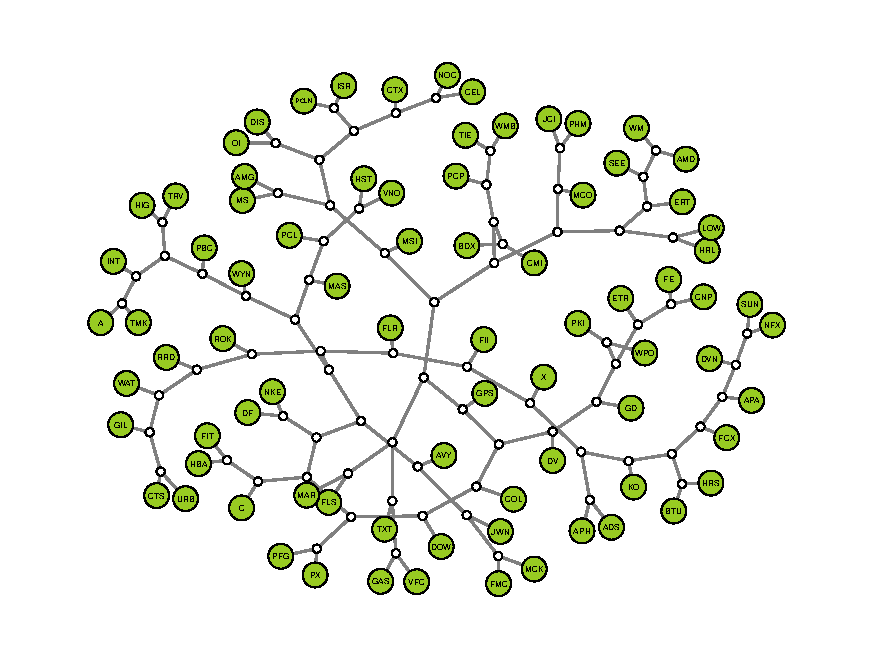
\includegraphics[scale=.8]{pics/structuralEM}
	\end{center}
\end{frame}

\subsection{High-dimensional Gaussian graphical models}

\begin{frame}[plain,noframenumbering]{}
\begin{center}
	{\huge \textcolor{DarkRed}{5.2 High-dimensional Gaussian graphical models}}
\end{center}
\end{frame}

\begin{frame}{Learning the graph in high-dimensions}
Let $Y=(X,H)$ be a \alert{Gaussian} vector with covariance $\Sigma$; $K=\Sigma^{-1}$.
\begin{alertblock}{Low-Rank Plus Sparse estimator}
 Then using standard matrix algebra
	$$
	(\Sigma_{XX})^{-1}=K_{XX}-K_{XH}K_{HH}^{-1}K_{HX}.
	$$
	If the graph of $Y$ is sparse then $K$ (and so also $K_{XX}$) is a sparse matrix. \\[.5cm]
	If the size of $H$ is small compared to $X$ then $K_{XH}K_{HH}^{-1}K_{HX}$ has small rank. \\[.5cm]
	Then $(\Sigma_{XX})^{-1}$ can be written as $S+L$, where $S$ is \textcolor{SeaGreen}{sparse} and $L$ is \textcolor{SeaGreen}{low rank}.
	\end{alertblock}	
\end{frame}

\begin{frame}{}
	Assuming that $(\Sigma_{XX})^{-1}=S+L$ where $S$ is sparse and $L$ has low rank, we can try to recover $S$ and $L$ using convex optimization techniques.  
	$$
	\mbox{maximize} \;\;\;\log\det(S+L)-{\rm tr}(W(S+L))\;+\;\lambda \|S\|_1\;+\;\gamma\|L\|_*,
	$$
where $W$ is the sample covariance matrix of the observed data, $\lambda, \gamma$ are positive constants, and $\|L\|_*=\sum_i \sigma_i(L)$ denotes the \alert{nuclear} norm of $L$. \\[.2cm]


The nuclear norm is a convex envelope of the rank function restricted to matrices with operator norm $\leq 1$. ({\footnotesize Details in the PhD thesis of Maryam Fazel ``Matrix rank minimization with applications'' (1435 Google citations)})
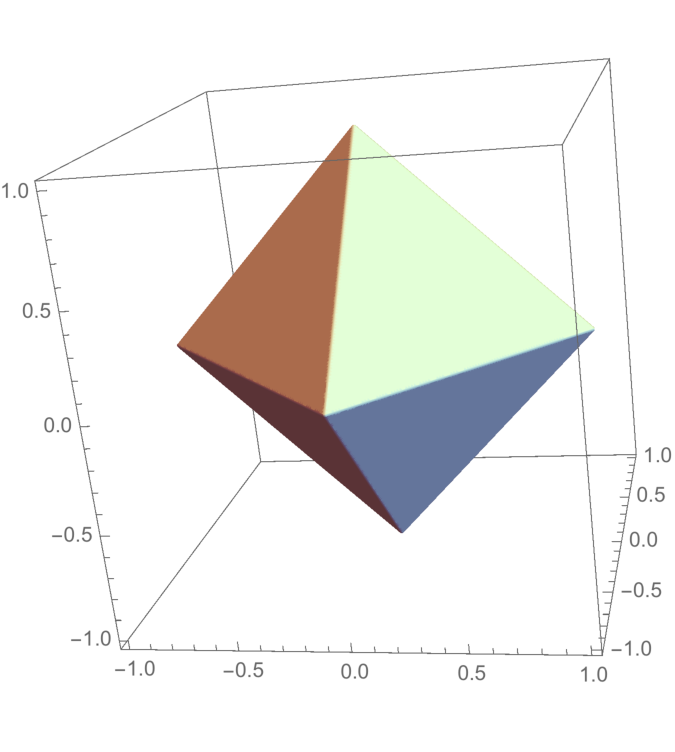
\includegraphics[scale=.3]{pics/lasso_ball}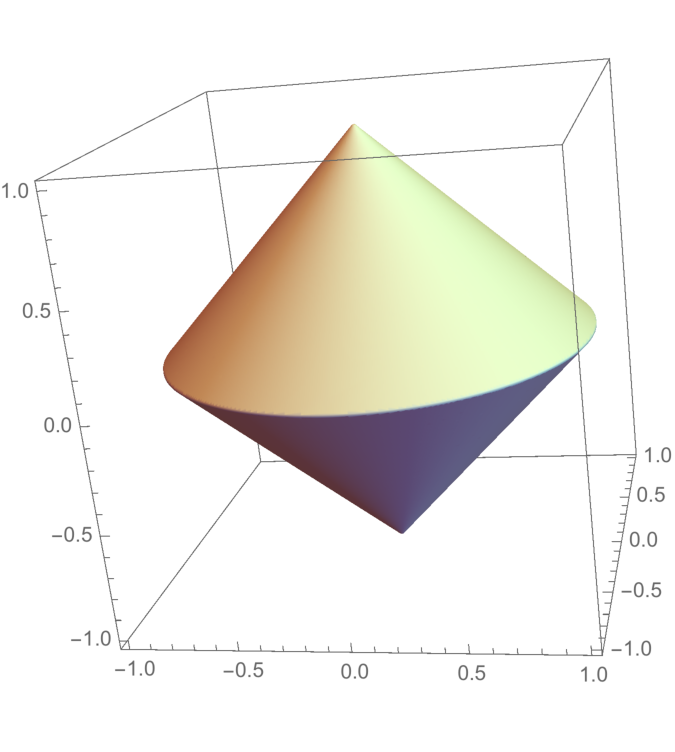
\includegraphics[scale=.3]{pics/glasso_ball}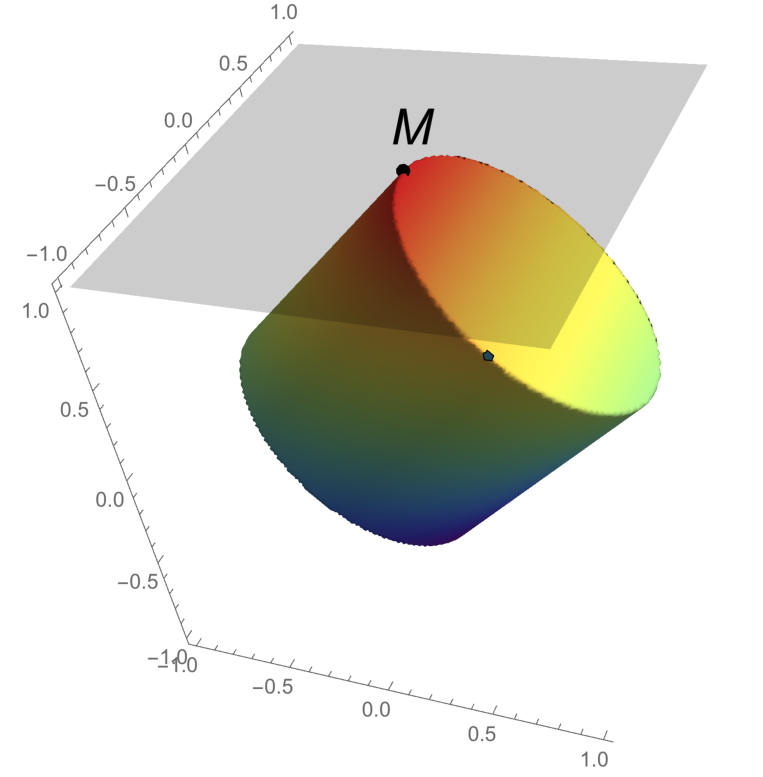
\includegraphics[scale=.25]{pics/nuclear}
\end{frame}

\begin{frame}[fragile]{Using an R implementation}
As an example study the stock data discussed earlier (c.f. Slide~\ref{SEM}).
	\begin{lstlisting}
install.packages("devtools"); library(devtools)
install_github("benjaminfrot/lrpsadmm")
library(lrpsadmm)
gammas <- c(0.1, 0.15, 0.2)
cvpath <- lrpsadmm.cv(dat, gammas = gammas,
                         lambda.ratio = 1e-02, n.lambdas = 30, verbose = TRUE)
best.gamma <- cvpath$best.gamma
best.lambda <- cvpath$best.lambda
best.fit <- cvpath$best.fit$fit
Khat <- -cov2cor(solve(best.fit$S)); diag(Khat) <- 1; rownames(Khat) <- colnames(Khat) <- stockdata$info[sample.stocks,1]
Khat <- -cov2cor(best.fit$S); diag(Khat) <- 1; rownames(Khat) <- colnames(Khat) <- stockdata$info[sample.stocks,1]
qgraph::qgraph(Khat,color="#98CB22",layout="spring",threshold=1e-3)
# plot according with nodes colored by economy segments
qgraph::qgraph(Khat,color=2*rank(stockdata$info[sample.stocks,2]),layout="spring",threshold=1e-3)
sum(abs(eigen(best.fit$L)$values)>1e-10) # gives that the rank of L is 16.
	\end{lstlisting}
	Some extensions to generalized linear models are forthcoming.
%# to get more information about the stocks
%> which(stockdata$info[,1]=="COG")
%[1] 70
%> stockdata$info[70,]
%               V1                V2                V3 
%            "COG"          "Energy" "Cabot Oil & Gas" 
\end{frame}

\begin{frame}{}
	\begin{center}
		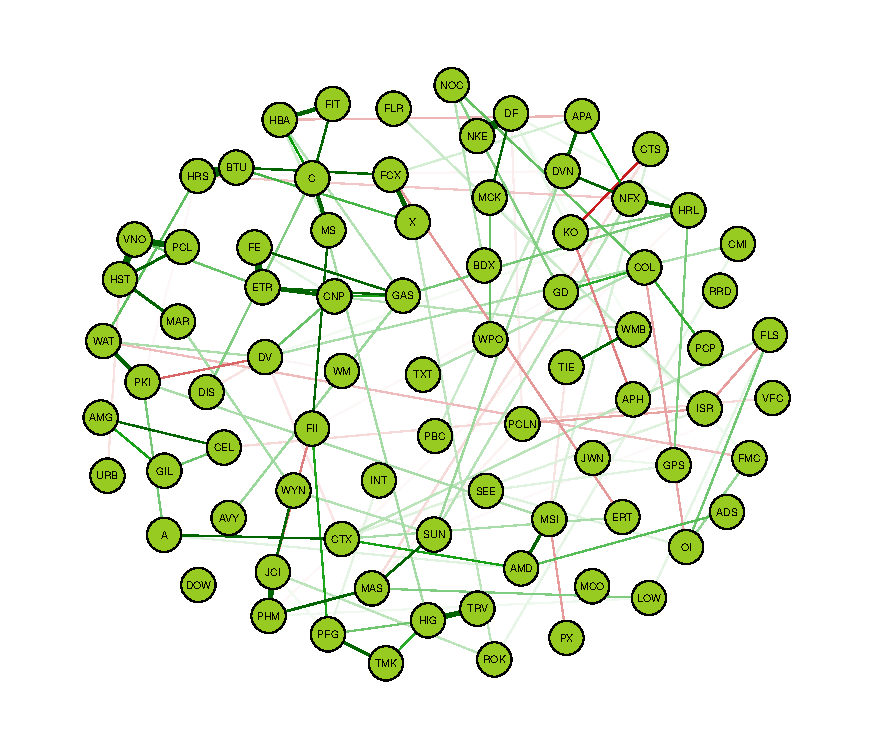
\includegraphics[scale=.85]{pics/stocks_latent}
	\end{center}
\end{frame}

%\begin{frame}{}
%Thresholding partial correlations $<0.05$ gives a very sparse graph.
%	\begin{center}
%		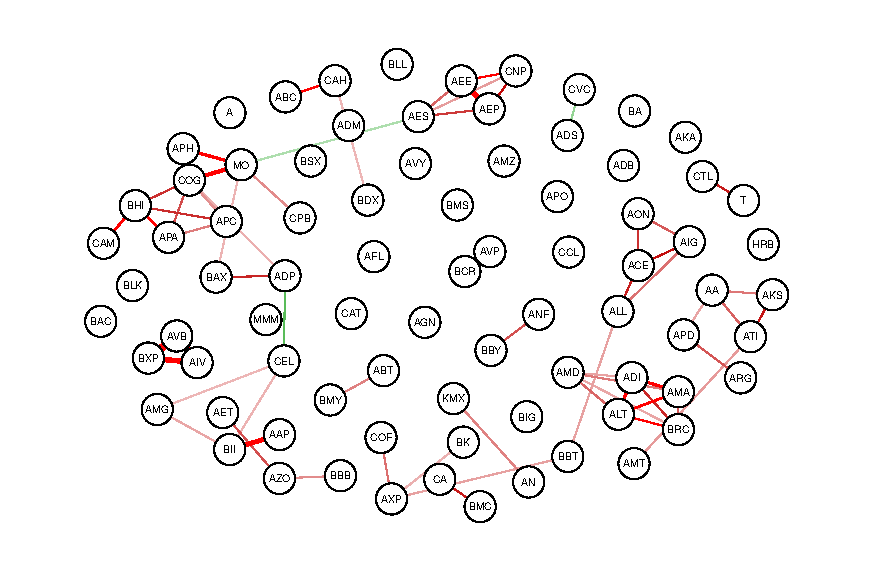
\includegraphics[scale=.9]{pics/stocks_latent2}
%	\end{center}
%\end{frame}

\subsection{Ancestral graphs}

\begin{frame}[plain,noframenumbering]{}
\begin{center}
	{\huge \textcolor{DarkRed}{5.3 Ancestral graphs}}
\end{center}
\end{frame}

\begin{frame}{Fix BNs for latent variables}
	Bayesian networks are not closed under taking margins.\\[.3cm]
		Maximal Ancestral Graphs (MAGs): the smallest family closed under taking margins and containing DAGs.\\[.2cm]
	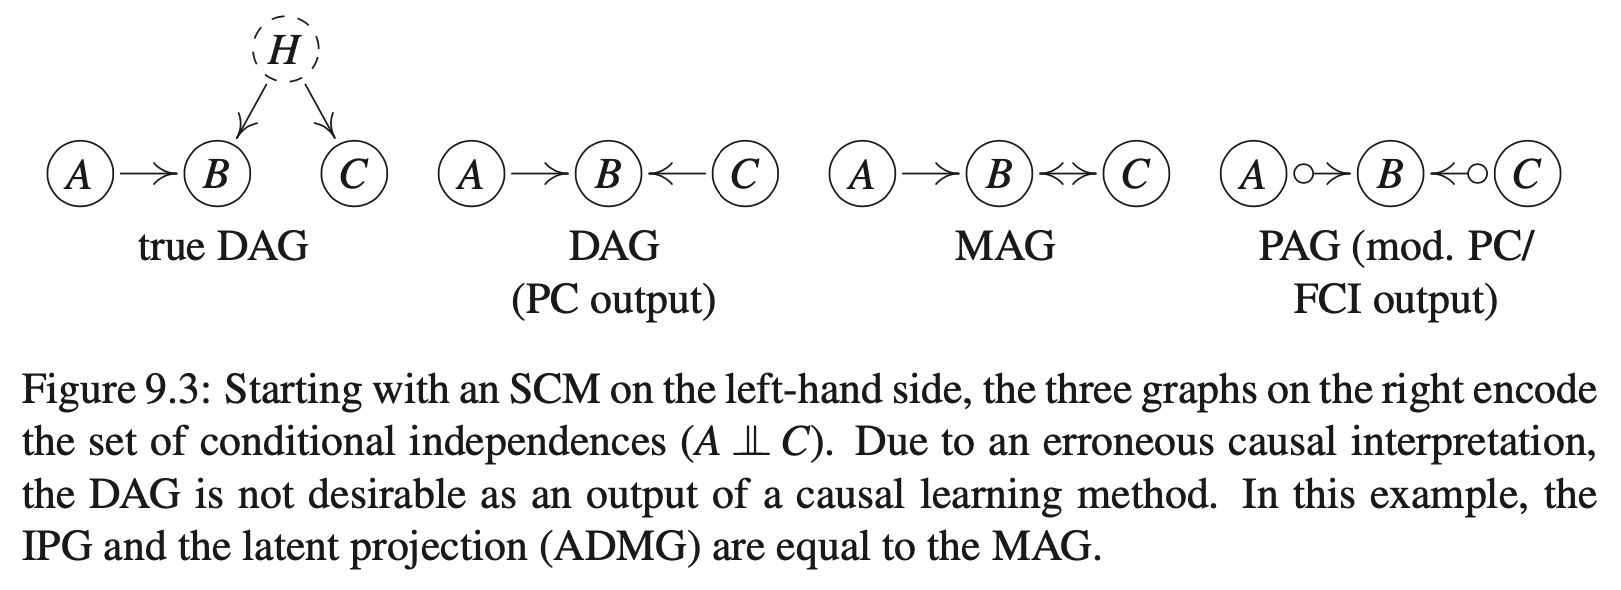
\includegraphics[width=\textwidth]{pics/ancestral}\\[.3cm]
PAG represents the equivalence class: 	$\circ$ in a PAG stands for ``either $-$ or $\to$''.
\end{frame}

%\begin{frame}{PAG: equivalence class of MAGs}
%	If $M$ is a $MAG$ then the graph $P$ representing its equivalence class:
%\begin{itemize}
%	\item Has the same skeleton as $M$. 
%	\item A mark of an arrowhead is in $P$ if and only if it lies in each equivalent MAG.
%\end{itemize}
%\end{frame}

\begin{frame}[fragile]{Example ancestral graph}
	\begin{lstlisting}
library(pcalg) 
data("gmG") 
p<-ncol(gmG$x)
suffStat<-list(C=cor(gmG$x),n=nrow(gmG$x)) 
G <- fci(suffStat , indepTest=gaussCItest , labels=nodes(gmG$g), skel.method="stable", alpha=0.01)
	\end{lstlisting}
	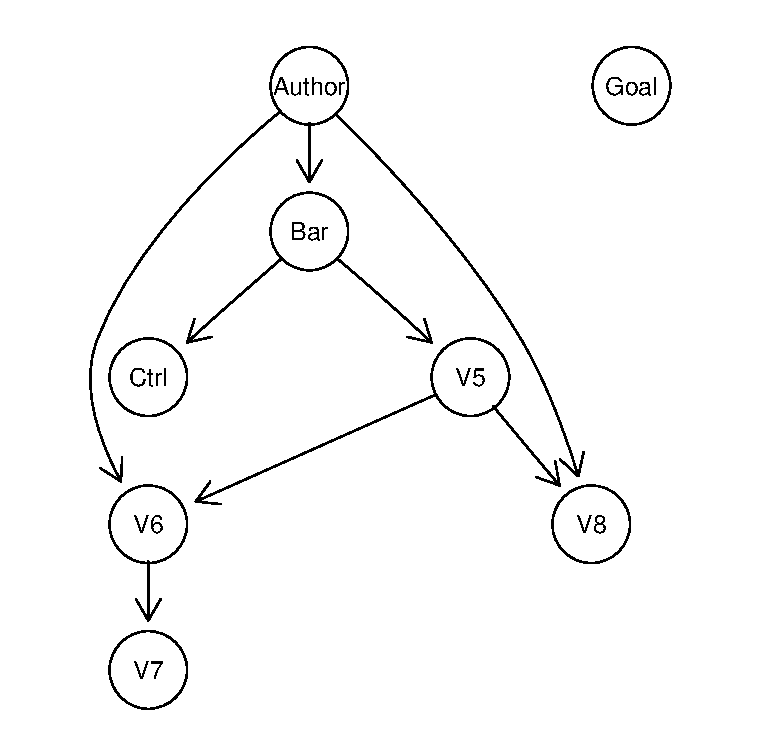
\includegraphics[width=.5\textwidth]{pics/fci_true}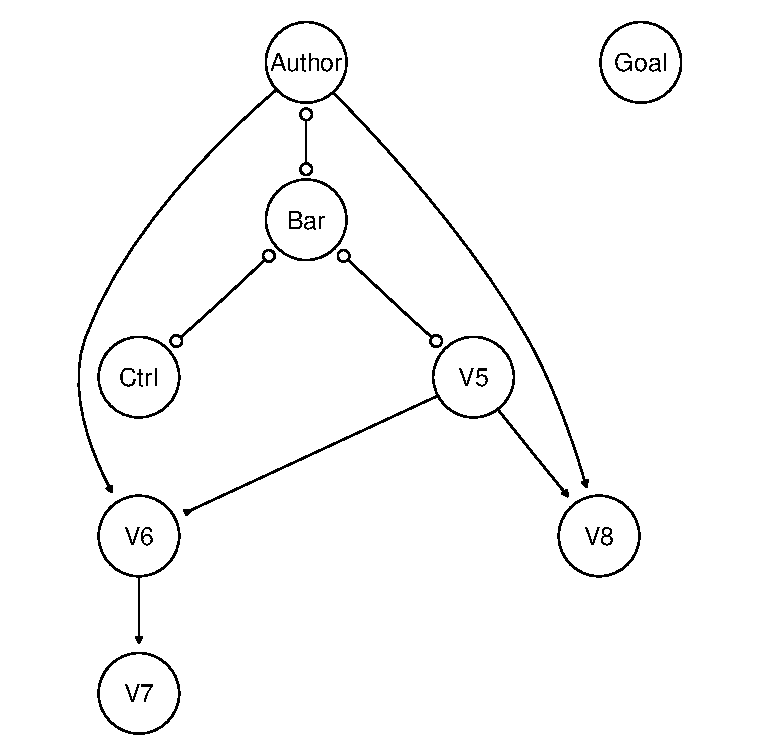
\includegraphics[width=.5\textwidth]{pics/fci_estimated}
\end{frame}



%\begin{frame}{Extensions to generalized linear models}
%	Amnir Taeb
%\end{frame}


%\section{Models for temporal data}
%\begin{frame}[plain,noframenumbering]{}
%\begin{center}
%	{\Huge \textcolor{DarkRed}{Part 5: Models for temporal data}}
%\end{center}
%\end{frame}

%\begin{frame}{Package \texttt{mgm}}
%	Estimation of k-Order time-varying Mixed Graphical Models and mixed VAR(p) models via elastic-net regularized neighborhood regression.
%\end{frame}


\section{Positive association}
\begin{frame}[plain,noframenumbering]{}
\begin{center}
	{\Huge \textcolor{DarkRed}{Part 6: Positive association}}
\end{center}
\end{frame}

\begin{frame}{Example 1: Two psychological disorders}
	\begin{center}
The sample correlations:\\[.3cm]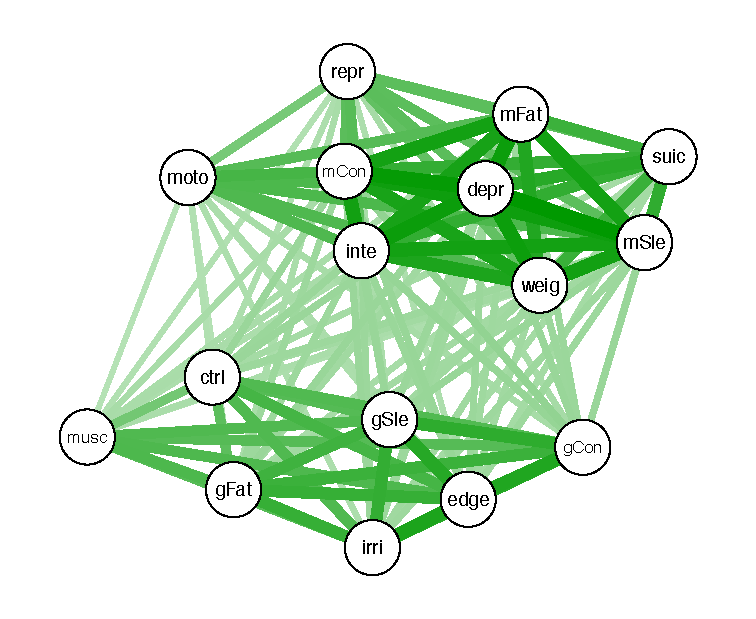
\includegraphics[scale=.6]{./pics/scorrdepr}.	
\end{center}
Note: All edges are green (positive sample correlations).
\end{frame}

\begin{frame}{}
	\begin{center}
$\ell1$-regularized Ising model:\\[.3cm]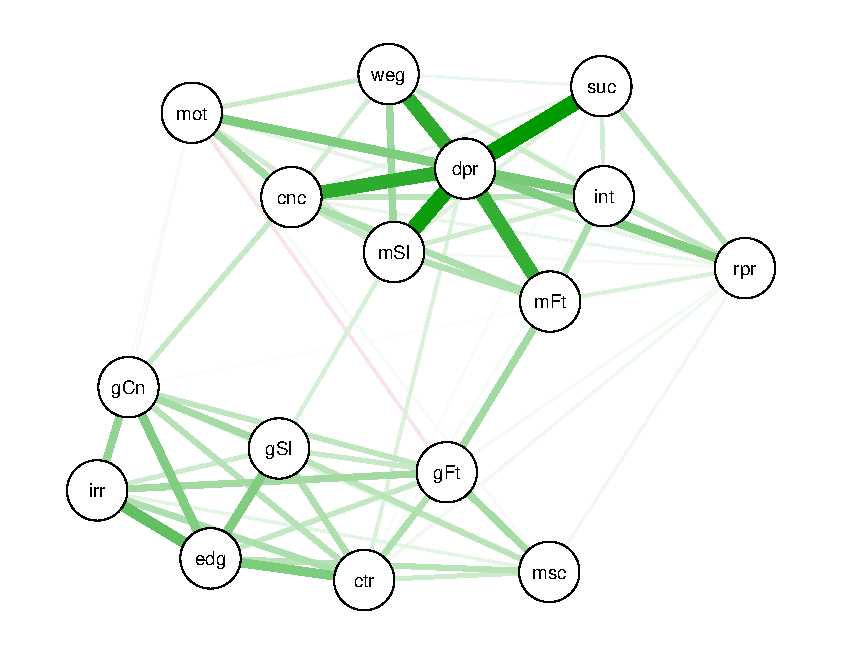
\includegraphics[scale=.6]{./pics/depr_lasso}.
\end{center}
Note: Most edges green (positive cond. log-odds ratios).
\end{frame}

\begin{frame}{Example 2: S\&P 500}
		\begin{center}
graphical lasso estimate of the graph:\\[.3cm]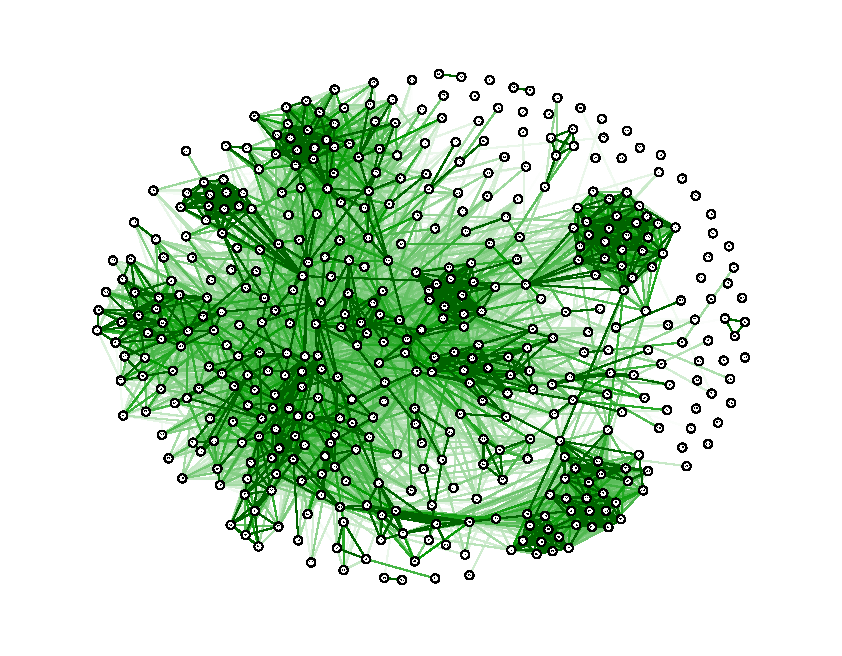
\includegraphics[scale=.6]{./pics/huge_stocks2}.
\end{center}
Note: All edges green (positive \alert{partial correlations}).
\end{frame}


\subsection{Basic concepts}

\begin{frame}[plain,noframenumbering]{}
\begin{center}
	{\huge \textcolor{DarkRed}{6.1 Basic concepts}}
\end{center}
\end{frame}


%\begin{frame}{Notation}
%%\begin{block}{}
%\begin{itemize}
%\item  $X=(X_{1},\ldots,X_{m})$,\quad $V:=\{1,\ldots,m\}$\\[.5cm]
%\item state space: $\cX=\prod_{i\in V} \cX_{i}$
%\begin{itemize}
%\item discrete case $\cX_{i}=\{0,\ldots,r_{i}-1\}$, or
%\item Gaussian case $\cX=\R^{m}$.\\[.5cm]
%\end{itemize}
%\item For $x,y\in \cX$ denote:
%\begin{itemize}
%\item \textcolor{blue}{$x\geq y$} \quad if $x_{i}\geq y_{i}$ for all $i=1,\ldots,m$,
%\item \textcolor{blue}{$x\wedge y$} \;\;=\;\; coordinatewise minimum
%\item \textcolor{blue}{$x\vee y$} \;\;=\;\; coordinatewise maximum
%\end{itemize}
%\end{itemize}
%%\end{block}
%%\begin{alertblock}{}
%%\begin{itemize}
%%\item probability \textcolor{blue}{density} function $p(x)$ on $\cX$
%%%\item in the discrete case $p\in \R^{\cX}=\R^{r_{1}\times \cdots\times r_{m}}$ is a \textcolor{blue}{tensor}
%%\begin{itemize}
%%\item sometimes \,\, \textcolor{blue}{$p_{x}$} \,\,for $p(x)$ if $\cX$ discrete
%%\item the underlying measure is a product measure.
%%\end{itemize}
%%\end{itemize}
%%\end{alertblock}
%\end{frame}


\begin{frame}
\frametitle{Definition}
	\begin{itemize}
\item $X=(X_{1},\ldots,X_{m})$, $\cX=\prod_{i=1}^m\cX_i\subset \R^m$, density $p$.\\[.7cm]
\item A function $p$  is \alert{$\mtp$} if:
$$
p(x)\,p(y)\;\;\leq\;\; p(x\wedge y)\,p(x\vee y)\qquad\mbox{for all }x,y\in \cX.
$$
\vspace{-.5cm}
\begin{itemize}
\item e.g. $p(1,1,0)p(0,0,1)\leq p(0,0,0)p(1,1,1)$\\[.7cm]
 \end{itemize}
% \item $X=(X_{1},\ldots,X_{m})$ is $\mtp$ if its distribution is.\\[.7cm] 
 \item If $p>0$ the condition simplifies.\\[.2cm]
\begin{itemize}
\item e.g. $p(1,1,0)p(0,1,1)\leq p(0,1,0)p(1,1,1)$\\[.7cm]
 \end{itemize}
 \end{itemize}
%\pause
\end{frame}

%\begin{frame}{Original motivation}
%	\begin{itemize}
%\item $X=(X_{1},\ldots,X_{m})$ is \alert{positively associated} if for any two \textit{non-decreasing} functions $\phi,\psi:\R^m\to \R$
%$${\rm corr}\{\phi(X),\psi(X)\}\geq 0.$$
%\end{itemize}	
%\vspace{.5cm}
%\begin{alertblock}{Theorem[FKG inequality]}
%	\qquad $\mtp$\qquad $\Longrightarrow$\qquad positively associated.	
%\end{alertblock}
%	\begin{itemize}
%\item e.g. ferromagnetic Ising models
%\end{itemize}
%{\scriptsize Fortuin, Kasteleyn, Ginibre, \textit{Correlation inequalities on some partially ordered sets}, 1971.}
%
%\end{frame}

\begin{frame}
\frametitle{Basic properties}
	\begin{itemize}
\item $X=(X_{1},\ldots,X_{m})$ is \alert{positively associated} if for any two \textit{non-decreasing} functions $\phi,\psi:\R^m\to \R$
$${\rm corr}\{\phi(X),\psi(X)\}\geq 0.$$
\end{itemize}	
If $X=(X_{1},\ldots,X_{m})$ is $\mtp$, then\\[.3cm]
\begin{itemize}
\item[(i)] any \textbf{marginal} distribution is $\mtp$;\\[.2cm]
\item[(ii)] any  \textbf{conditional} distribution is $\mtp$;\\[.2cm]
\item [(iii)] $X$ is associated.
\end{itemize}
\vspace{.7cm}
{\footnotesize S. Karlin, Y. Rinott, \textit{Classes of orderings of measures and related correlation inequalities. I. Multivariate totally positive distributions}, JMVA, 1980.}
%\bigskip
%
%\alert{There is no Yule-Simpson paradox!}
%\pause
%\pause
%\begin{itemize}
%	\item Independence structure for $\mtp$ vector $X=(X_1,\ldots,X_m)$
%\begin{itemize}
%\item $X_{i}\indep X_{j}$ if and only if ${\rm cov}(X_{i},X_{j})=0$.
%\item $X$ can be split into independent blocks and within each block all covariances are \alert{strictly} positive.
%\end{itemize}
%\vspace{.2cm}
%%\pause
%\item Conditional independence structure: for example \alert{upward stability} 
%\begin{itemize}
%\item $X_{A}\indep X_{B}|X_{C}$ implies $X_{A}\indep X_{B}|X_{C\cup \{k\}}$
%\item see also: K. Sadeghi, \textit{Faithfulness of Probability Distributions and Graphs}, JMLR 2017.  
%\end{itemize}
%\end{itemize}
 \end{frame}



%\begin{frame}{Conditional independence structure}
%\begin{block}{}
%In [\alert{\small S. Fallat, et al, Total positivity in Markov structures, AoS,  2017}] we studied Markov structures of $\mtp$ distributions.
%\end{block}
%
%	\begin{itemize}
%	\item Independence structure
%\begin{itemize}
%\item ${\rm cov}(X_{i},X_{j})=0$ implies that $X_{i}$ independent of $X_{j}$.
%\item $X$ can be split into independent blocks and within each block all covariances are \alert{strictly} positive.
%\end{itemize}
%\vspace{.2cm}
%%\pause
%\item Conditional independence structure: for example \alert{upward stability} 
%\begin{itemize}
%\item $X_{A}\indep X_{B}|X_{C}$ implies $X_{A}\indep X_{B}|X_{C\cup \{k\}}$
%\item see also: K. Sadeghi, \textit{Faithfulness of Probability Distributions and Graphs}, JMLR 2017.  
%\end{itemize}
%\end{itemize}
%\end{frame}


%\begin{frame}[plain,noframenumbering]{}
%\begin{center}
%	{\huge \textcolor{DarkRed}{Gaussian $\mtp$}}
%\end{center}
%\end{frame}

\begin{frame}{Two special cases}
\begin{beamercolorbox}[wd=\paperwidth,sep=5pt]{result}
	\alert{Gaussian model}: $f(x)\;=\;\tfrac{1}{(2\pi)^{p/2}}\sqrt{\det K}\exp(-x^T\!K\,x/2)$\\[.2cm]
$\mtp$ \quad$\Longleftrightarrow$\quad $K=\Sigma^{-1}$ satisfies $K_{ij}\leq 0$ for all $i\neq j$.
\end{beamercolorbox}
\bigskip
\begin{beamercolorbox}[wd=\paperwidth,sep=5pt]{result}
	\alert{Binary Ising model}: $f(x)\;=\;\tfrac{1}{Z(h,J)}\exp(h^Tx+x^T\!J\,x/2)$\\[.2cm]
$\mtp$ \quad$\Longleftrightarrow$\quad $J_{ij}\geq 0$ for all $i\neq j$.
\end{beamercolorbox}
\end{frame}



%\begin{frame}{Our motivation}
%	\begin{itemize}
%		\item Useful concept in data modelling.\\[.7cm]
%		\item Some popular models are implicitly $\mtp$.\\[.7cm]
%		\item Interesting new results for \alert{attractive} GMs.\\[.7cm]
%		\item Leads to sparsity, applies in high-dimensions. \\[.7cm]
%	\end{itemize}
%\end{frame}


\subsection{Modelling}
\begin{frame}[plain,noframenumbering]{}
\begin{center}
	{\huge \textcolor{DarkRed}{6.3 Modelling}}
\end{center}
\end{frame}


\begin{frame}
\frametitle{A restrictive condition?}
\begin{itemize}
\item $\mtp$ contraints appear to be \textit{restrictive}:
\begin{itemize}
\item  $3$-dim Gaussian: about $5\%$ of distributions are $\mtp$,
\item  $4$-dim Gaussian: about $0{.}09\%$ of distributions are $\mtp$.\\[.4cm]
\end{itemize}
%\item $\mtp$ distributions are \textit{abundant} in real data
\item Less restrictive under additional Markov structure.\\[.4cm]
\item In the $3$-dim case
\begin{itemize}
\item if $1\indep 2|3$  then $25\%$ are $\mtp$
\item if, in addition, $1\indep 3|2$ then $50\%$ are $\mtp$
\item if $1\indep 2\indep 3$  then everything is $\mtp$\\[.4cm]
\end{itemize}
\end{itemize}
Informally: In sparse structures $\mtp$ is more likely.\\[.1cm]
%{\tiny(*)}{\TINY It is more likely to see $\mtp$ distribution in sparse structures especially in settings where total positivity is expected. }
\end{frame}

\begin{frame}
\frametitle{Example 3: EPH-gestosis}
{\footnotesize \begin{itemize}
	\item Dataset collected 45 years ago in a study on ``Pregnancy and Child Development'' %by the German Research Foundation  
\item {EPH-gestosis (pre-eclampsia):} disease \textbf{syndrome} for pregnant women; three \textbf{symptoms} (high body water retention, high amounts of urinary proteins, elevated blood pressure)
%\begin{itemize}
%\item edema (high body water retention)
%\item proteinuria (high amounts of urinary proteins) 
%\item hypertension (elevated blood pressure)
%\end{itemize}	
\item A {syndrome} is a set of medical signs and symptoms that are {correlated} with each other and, often, with a particular disease or disorder. 
%The word derives from the Greek and means \textbf{"concurrence"}. (Wikipedia)
\end{itemize}	}

\begin{beamercolorbox}[wd=\paperwidth,sep=5pt]{result}
	%	\begin{itemize}
%		\item Observed counts:
%\vspace{-.2cm}
{\footnotesize The sample distribution$$
\left[\begin{array}{cccc}
\hat p_{000} & \hat p_{010} & \hat p_{001} & \hat p_{011} \\
\hat p_{100} & \hat p_{110} & \hat p_{101} & \hat p_{111} 
\end{array}\right]= \tfrac{1}{4649}\left[\begin{array}{cccc}
3299 & 107 & 1012 & 58 \\
78 & 11 & 65 & 19
\end{array}\right]
$$
is already $\mtp$. \underline{Equivalently}, $X_1\indep X_2\indep X_3|H$ for a latent binary $H$.}
\end{beamercolorbox}
%\item This sample distribution is $\mtp$.
%\begin{itemize}
%\item \alert{equivalently}: $X_1\indep X_2\indep X_3|H$ for some binary $H$
%	\end{itemize}
%	\end{itemize}
\end{frame}

\begin{frame}{Example 4: Financial time series.}
	Monthly correlations of global stock markets
	{\footnotesize$$
S = \bordermatrix{~ & Nasdaq & Canada & Europe & UK &Australia \cr
              Nasdaq &    1.000 & 0.606 & 0.731 & 0.618 &0.613\cr
              Canada &    0.606 & 1.000 & 0.550 & 0.661 &0.598\cr
              Europe &    0.731 & 0.550 & 1.000 & 0.644 &0.569\cr
              UK &        0.618 & 0.661 & 0.644 & 1.000 &0.615\cr
              Australia & 0.613 & 0.598 & 0.569 & 0.615 &1.000\cr
              }
$$}
{\footnotesize$$
S^{-1} = \bordermatrix{~ & Nasdaq & Canada & Europe & UK &Australia \cr
              Nasdaq &    2.629 & -0.480 & -1.249 & -0.202 &-0.490\cr
              Canada &    -0.480 & 2.109 & -0.039 & -0.790 &-0.459\cr
              Europe &    -1.249 & -0.039 & 2.491 & -0.675 &-0.213\cr
              UK &        -0.202 & -0.790 & -0.675 & 2.378 &-0.482\cr
              Australia & -0.490 & -0.459 & -0.213 & -0.482 &1.992\cr
              }
$$}
Sampled uniformly this happens with prob. $<10^{-6}$!
\end{frame}

\begin{frame}{Example 5: Math grades}
Data:  grades of 88 students in
\texttt{Mechanics, Vectors, Algebra, Analysis, Statistics}
%\vspace{-.2cm}
%\begin{scriptsize}
{\footnotesize$$
S = \bordermatrix{~ & mechanics & vectors & algebra & analysis & statistics \cr
              mechanics &    305.7680 & 127.2226 &101.5794 & 106.2727  & 117.4049\cr
              vectors &    127.2226 & 172.8422 & 85.1573  & 94.6729   & 99.0120\cr
              algebra &    101.5794  & 85.1573 & 112.8860 & 112.1134  & 121.8706\cr
              analysis &        106.2727&  94.6729& 112.1134& 220.3804&  155.5355\cr
              statistics & 117.4049&  99.0120 & 121.8706& 155.5355&  297.7554 \cr
              }
$$}
{\footnotesize$$
S^{-1} = \bordermatrix{~ & mechanics & vectors & algebra & analysis & statistics \cr
              mechanics &    5.2446& -2.4351& -2.7395&  \textcolor{Important}{0.0116}& -0.1430\cr
              vectors &    -2.4351 & 10.4268 &-4.7078 &-0.7928 & -0.1660\cr
              algebra &    -2.7395 &-4.7078 & 26.9548 &-7.0486 &-4.7050\cr
              analysis &        \textcolor{Important}{0.0116} &-0.7928 &-7.0486&  9.8829& -2.0184 \cr
              statistics & -0.1430 & -0.1660 & -4.7050 &-2.0184 & 6.4501\cr
              }
$$}
\end{frame}


%\begin{framefont}{\scriptsize}
\begin{frame}{$\mtp$ constraints are often explicit}
\vspace{-.5cm}\begin{center}
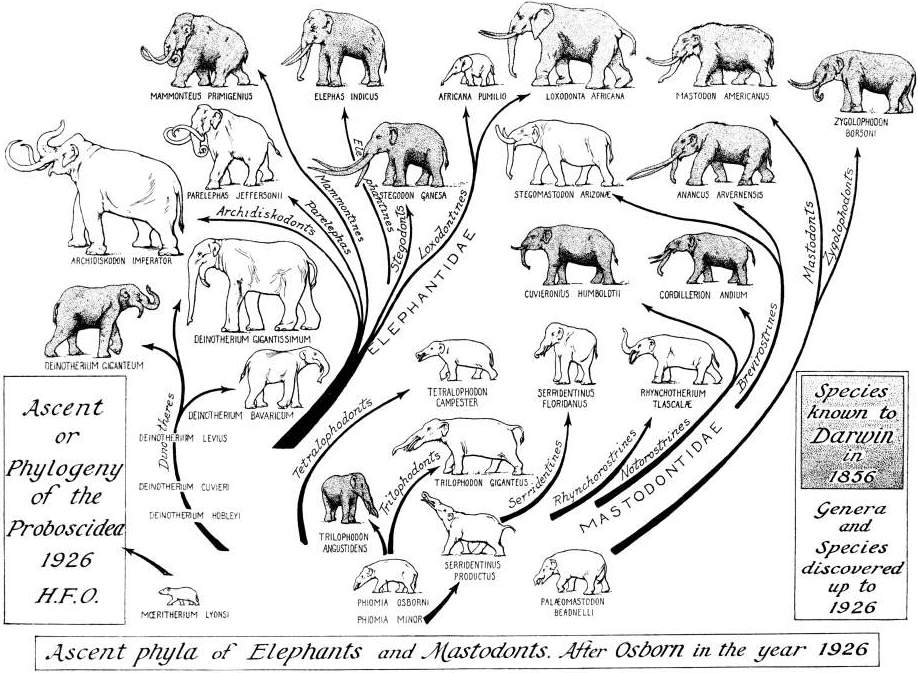
\includegraphics[scale=.25]{./pics/phylo_elephants}	
\end{center}\vspace{-.3cm}
	\begin{minipage}{6cm}{\scriptsize
		$X$ is $\mtp$ in:
		\begin{itemize}
			\item ferromagnetic Ising models
			\item Markov chains with $\mtp$ transitions
			\item order statistics of \emph{iid} variables
			\item Brownian motion tree model
		\end{itemize}}
	\end{minipage}\begin{minipage}{6cm}
		{\scriptsize $|X|$ is $\mtp$ in:
		\begin{itemize}
			\item Gaussian/binary tree models
			\item Gaussian/binary latent tree models
			\begin{itemize}
			\item {\scriptsize binary latent class models}
			\item {\scriptsize single factor analysis models}
			\end{itemize}
		\end{itemize}}
	\end{minipage}
\end{frame}
%\end{framefont}

%
%
%\begin{frame}
%\frametitle{Signed $\mtp$ distributions}
%\begin{itemize}
%\item Definition: A Gaussian r.v. $X=(X_1,\ldots,X_m)$ has a \alert{signed $\mtp$} distribution if there exists a diagonal matrix $D\in \{-1,+1\}^m$ such that $DX$ has an $\mtp$ distribution.
%\end{itemize}
%\begin{alertblock}{Theorem (LUZ 2016):}
%	\begin{itemize}
%	\item  Every Gaussian \alert{model on a tree} is signed $\mtp$.
%	\item Signed $\mtp$ property is preserved under taking margins.
%	\begin{itemize}
%		\item single factor analysis models, Gaussian latent tree models, binary latent class models, and binary latent tree models 
%	\end{itemize}
%	\end{itemize}
%	\end{alertblock}
%	\pause
%	\begin{block}{}
%	\begin{itemize}
%		\item Most of the results that I am going to present directly extend from $\mtp$ to signed $\mtp$ distributions.
%	\end{itemize}
%	\end{block}
%\end{frame}
%
%




%\begin{frame}
%\frametitle{Exponential family}
%\begin{itemize}
%\item  
%$p(x;\theta)=g(x)\exp(\langle \theta,T(x)\rangle -A(\theta))$, \quad $\theta\in C\subseteq \R^{d}$, $x\in \cX$.
%\begin{itemize}
%\item (sufficient statistics) $T:\,\cX\to \R^{d}$
%\item (\alert{canonical parameters}) $C=\{\theta:\, \int \exp(\langle \theta,T(x)\rangle)\nu({\rm d}x)<\infty\}$
%\end{itemize}
%\item $C$ is convex and $A(\theta)$ is strictly convex in $C$
%\end{itemize}
%\pause 
%\begin{itemize}
%\item $x^{(1)},\ldots,x^{(n)}\in \cX$ independent sample;\quad $\bar T:=\tfrac{1}{n} \sum_i T(x^{(i)})$
%\item the log-likelihood function:\quad $\ell(\theta)=n\langle \theta,\bar T\rangle -nA(\theta)$
%\item $\ell$ strictly concave in $C$ and so the MLE is unique (if exists) 
%\end{itemize}
%\pause
%\begin{itemize}
%\item \textbf{Theorem (LUZ)}:  The set of all $\theta\in C$ such that $p(x;\theta)$ is $\mtp$ is an intersection of $C$ with a closed \textcolor{Important}{convex} set $\Gamma$. For graphical models $\Gamma$ is a \alert{non-empty polyhedral}    cone.
%\begin{itemize}
%\item the MLE is unique
%\item the boundary decomposes into smaller $\mtp$ exponential families
%\end{itemize}
%\end{itemize}
%\end{frame}

%\begin{frame}
%\frametitle{The maximum likelihood estimator}
%%\begin{itemize}
%\item  $p(x)=g(x)\exp(\langle \theta,T(x)\rangle -A(\theta))$, $\theta\in C\subseteq \R^{d}$, $x\in \cX$.
%\end{itemize}
%%%\begin{itemize}
%\item $x^{(1)},\ldots,x^{(n)}\in \cX$ independent data;\quad $\bar T:=\tfrac{1}{n} T(x^{(i)})$
%\item the log-likelihood function:\quad $\ell(\theta)=n\langle \theta,\bar T\rangle -nA(\theta)$
%\item $\ell$ strictly concave in $C$ and so the MLE is unique (if exists) 
%\end{itemize}
%%%\begin{itemize}
%\item MLE exists \quad if and only if \quad$\bar T\in {\rm int}(K)$.
%\item It is given by the unique point in the preimage of $-\nabla A(\theta)$.
%\end{itemize}
%%\end{frame}

%\begin{frame}
%\frametitle{$\mtp$ exponential family}
%%\begin{itemize}
%\item Describe all $\theta\in C$ such that $p(x;\theta)$ is $\mtp$.
%\item \textbf{Proposition}: It is an intersection of $C$ with a relatively closed convex set $\Gamma$.
%\begin{itemize}
%\item Remark: Typically $\Gamma$ is a cone. 
%\end{itemize}
%\end{itemize}
%%%Proof sketch:
%\begin{itemize}
%\item check $\Delta(x,y;\theta)=\log\left(\tfrac{p(x\wedge y;\theta)p(x\vee y;\theta)}{p(x;\theta)p(y;\theta)}\right)\geq 0$ for all $x,y$
%\item $\Delta(x,y;\theta)$ is linear in $\theta$
%\end{itemize}
%%%\begin{itemize}
%\item \textbf{Theorem}: For graphical models $\Gamma$ is non-empty and polyhedral.
%\end{itemize}
%%{\tiny joint work with Steffen Lauritzen and Caroline Uhler; soon to be on arXiv}
%\end{frame}
%
%\begin{frame}
%\frametitle{Quadratic families}
%%\begin{itemize}
%\item $p(x)=\exp(-\sum_{i,j=1}^{m}\theta_{ij}x_{i}x_{j}-A(\theta))$
%\end{itemize}
%%%\begin{itemize}
%\item Proposition: A quadratic exponential family is $\mtp$ if and only if $\theta_{ij}\leq 0$ for all $i\neq j$.
%\item The parameter space is the negative orthant.
%\item The boundary corresponds to some sparse submodels.
%\end{itemize}
%%%\begin{itemize}
%\item Theorem: The maximum likelihood exists as long as the sample size $\geq 2$. In particular, the MLE estimator makes sense also in the high dimensional setting. 
%\end{itemize}
%%\end{frame}
%
%



%\begin{frame}
%\frametitle{Example: Gaussian $\mtp$ distributions}
%%\begin{itemize}
%\item ${\rm PD}_{m}=$ symmetric $m\times m$ positive definite matrices 
%\item $m$-dimensional \alert{Gaussian distribution} with covariance $\Sigma\in {\rm PD}_{m}$ 
%\item concentration matrix $K:=\Sigma^{-1}$
%\item Gaussian $X$ is $\mtp$ if and only if $K_{ij}\leq 0$ for all $i\neq j$
%\end{itemize}
%%%\begin{itemize}
%\item \textit{i.i.d.} data: $x^{(1)},\ldots,x^{(n)}\in \R^{m}$
%\item sample covariance matrix: $S=\tfrac{1}{n}\sum_{i} x^{(i)}(x^{(i)})^{T}$
%\item the \alert{log-likelihood function}: $\ell(K)=\log\det K-{\rm tr}(SK)$
%\end{itemize}
%%\end{frame}

%\begin{frame}[plain,noframenumbering]{}
%\begin{center}
%	{\huge \textcolor{DarkRed}{Sparse structures}}
%\end{center}
%\end{frame}

\begin{frame}{Recall: Two special cases}
\begin{beamercolorbox}[wd=\paperwidth,sep=5pt]{result}
	\alert{Gaussian model}: $f(x)\;=\;\tfrac{1}{(2\pi)^{p/2}}\sqrt{\det K}\exp(-x^T\!K\,x/2)$\\[.2cm]
$\mtp$ \quad$\Longleftrightarrow$\quad $K=\Sigma^{-1}$ satisfies $K_{ij}\leq 0$ for all $i\neq j$.
%\medskip
%\begin{itemize}
%	\item $K_{ij}\leq 0$ if and only if ${\rm corr}(X_i,X_j|X_{V\setminus \{i,j\}})\geq 0$.\\[.3cm]
%	\item ${\rm corr}(X_i,X_j|X_{A})\geq 0$ for every $A\subseteq V\setminus \{i,j\}$.
%\end{itemize}	
\end{beamercolorbox}
\medskip
\begin{beamercolorbox}[wd=\paperwidth,sep=5pt]{result}
	\alert{Binary Ising model}: $f(x)\;=\;\tfrac{1}{Z(h,J)}\exp(h^Tx+x^T\!J\,x/2)$\\[.2cm]
$\mtp$ \quad$\Longleftrightarrow$\quad $J_{ij}\geq 0$ for all $i\neq j$.
%\medskip
%\begin{itemize}
%	\item $K_{ij}\leq 0$ if and only if ${\rm corr}(X_i,X_j|X_{V\setminus \{i,j\}})\geq 0$.\\[.3cm]
%	\item ${\rm corr}(X_i,X_j|X_{A})\geq 0$ for every $A\subseteq V\setminus \{i,j\}$.
%\end{itemize}	
\end{beamercolorbox}

\bigskip
Convex constraint on the space of the (canonical) parameters with the boundary given by zeros. \\[.3cm]
Informally: In estimation $\mtp$ leads to sparsity.
\end{frame}


\begin{frame}[plain,noframenumbering]{}
\begin{center}
	{\huge \textcolor{DarkRed}{4.2 Gaussian models and finance}}
\end{center}
\end{frame}



\begin{frame}
\frametitle{MLE for Gaussian models}
\begin{itemize}
\item ${\rm maximize}\{\log\det K-{\rm tr}(SK)\}$ over $K\in \mtp$.\\[.5cm]
%\item Dual:  maximize \alert{$\log\det \Sigma$} subject to:
%\begin{itemize}
%\item $\Sigma_{vv}=S_{vv}$ for all $v\in V$
%\item $\Sigma_{uv}\geq S_{uv}$ for all $u\neq v$
%\item $\Sigma\in {\rm PD}_m$
%\end{itemize}
\item The MLE exists iff there exists $\,\Sigma\in {\rm PD}_m$ with $\Sigma\geq S$. \\[.5cm]
\item It is the unique element $\,\hat K = \hat{\Sigma}^{-1}\in {\rm PD}_m$ that satisfies
\begin{itemize}
\item \alert{Primal feasibility:} \;$\hat K_{ij}\leq0\;\; \forall i\neq j,$
\item \alert{Dual feasibility:} \quad $\hat\Sigma_{ii}=S_{ii}\;\; \forall i, \quad \hat\Sigma_{ij}\geq S_{ij}\;\; \forall i\neq j$
%\item[(c)] \alert{Stationarity of Lagrangian:} \, $\tr(S\hat\theta)= m$,
\item \alert{Complimentary slackness:} \;\; $(\hat\Sigma_{ij}-S_{ij}) \,\hat K_{ij}= 0 \;\; \forall i\neq j$.
\end{itemize}
\end{itemize}
\begin{beamercolorbox}[wd=\paperwidth,sep=5pt]{important}
	Note: \,\,\, We get zeros in $\hat K$ for free.
\end{beamercolorbox}
\end{frame}


%\begin{frame}{Single-linkage matrix}
%Let $S$ be the sample \emph{correlation} matrix. Assume $S_{ij}\geq 0$ for all $i\neq j$. \\[.5cm]
%	Given the weighted graph of $S$, the single-linkage matrix $Z$ is
%	$$
%	Z_{ij}\;=\;\max_{P\in \mathcal P(i,j)}\min_{uv\in P} S_{uv}\qquad\mbox{for }i\neq j.
%	$$
%	\vspace{-.6cm}
%	\begin{block}{}
%	$\bullet$\;\;	$Z$ is both primarly and dually feasible.
%	\end{block}
%	The fact that $Z\geq S$ (dual feasibility) is easy to establish.\\[.5cm]
%	The fact that $Z^{-1}$ is an M-matrix (primal feasibility) uses the connection to ultrametric matrices:
%	\begin{itemize}
%		\item Proposition: If $S_{ij}<1$ for all $i\neq j$, then $Z$ is non-singular and $Z^{-1}$ is an M-matrix.
%		\item see also: Dellacherie, Martinez, San Martin, \textit{Inverse M-matrices and ultrametric matrices}, Springer,  2014.
%	\end{itemize} 
%\end{frame}
%
%\begin{frame}{Example}
%	Suppose that 
%	$$
%	S\;=\;\begin{bmatrix}
%		1 &-0.5 &0.5 &0.6 \\
%		 -0.5&1 &0.4 &-0.1 \\
%		 0.5& 0.4& 1& 0.2\\
%		 0.6&-0.1 & 0.2&1 		
%	\end{bmatrix}
%	$$
%	Then $Z$ is given by	
%
%\qquad\qquad\begin{minipage}{0.4\textwidth}
%\begin{tikzpicture}[auto, node distance=2cm, every loop/.style={},
%                    main node/.style={circle,draw,font=\large}]
%
%  \node[main node] (1) {1};
%  \node[main node] (2) [below left of=1] {2};
%  \node[main node] (3) [below right of=2] {3};
%  \node[main node] (4) [below right of=1] {4};
%
%  \path[every node/.style={}]
%    (1) edge node [right] {0.6} (4)
%        edge [right] node[left] {0.5} (3)
%    (2) edge [right] node[left] {0.4} (3)
%    (3) edge [right] node[right] {0.2} (4);
%\end{tikzpicture}
%\end{minipage} 
%\begin{minipage}{0.3\textwidth}
%$$
%	Z\;=\;\begin{bmatrix}
%		1 &0.4 &0.5 &0.6 \\
%		 0.4&1 &0.4 &0.4 \\
%		 0.5& 0.4& 1& 0.5\\
%		 0.6&0.4 & 0.5&1 		
%	\end{bmatrix}.
%	$$
%\end{minipage}
%\smallskip
%
%%\begin{beamercolorbox}[wd=\paperwidth,sep=9pt]{notabene}	
%%The maximum cost spanning tree of $S$ plays an important role here. 
%%\end{beamercolorbox}
%\end{frame}


%\begin{frame}
%\frametitle{Example: Carcass data}
%\begin{itemize}
%\item data: thickness of meat and fat layers at different locations on the back of a slaughter pig on each of 344 carcasses 
%\end{itemize}
%$$
%S=\begin{blockarray}{ccccccc}
%\textrm{Fat11} & \textrm{Meat11} & \textrm{Fat12} & \textrm{Meat12} & \textrm{Fat13}&\textrm{Meat13} \\
%\begin{block}{(rrrrrr)l}
%1 & 0.04 & \colorbox{blue!20!white}{0.84} & 0.08 & 0.82 & \textcolor{Important}{-0.03}&\textrm{Fat11}\\ 
%\cdot & 1 & 0.04 & \colorbox{blue!20!white}{0.87} & \colorbox{blue!20!white}{0.13} & 0.86& \textrm{Meat11} \\
%\cdot& \cdot & 1 & 0.01 & \colorbox{blue!20!white}{0.83} & \textcolor{Important}{-0.03}&\textrm{Fat12}\\
%\cdot & \cdot & \cdot & 1 & 0.11 & \colorbox{blue!20!white}{0.90}& \textrm{Meat12} \\
%\cdot & \cdot & \cdot & \cdot & 1& 0.02&\textrm{Fat13} \\
%\cdot & \cdot & \cdot & \cdot & \cdot & 1&\textrm{Meat13} \\
%\end{block}
%\end{blockarray}
%$$
%\begin{itemize}
%	\item Spanning tree: Fat11---Fat12---Fat13---Meat11---Meat12---Meat13
%\end{itemize}
%\end{frame}
%
%
%\begin{frame}
%\frametitle{Example: Carcass data (2)}
%\begin{center}
%\includegraphics[width=4.2cm]{Carcass_MTP2_graph2.pdf}
%\begin{center}
%$\mtp$ constraint
%\end{center}
%\end{center}
%\begin{itemize}
%	\item Only one non-edge satisfies $S_{ij}\geq \prod_{uv\in \overline{ij}}S_{uv}$.
%\end{itemize}
%\end{frame}

%\begin{frame}
%\frametitle{Existence of the MLE}
%Learning sparse structures in high dimensions was the main motivation of {\scriptsize [\alert{Slawski, Hein, \textit{Estimation of positive definite M-matrices and structure learning for attractive Gaussian Markov random fields}, 2015}]}.	\\[.5cm]
%
%\textbf{Theorem (Slawski,Hein(2015))}: The MLE exists with \textit{probability one} for sample size $n\geq 2$.\\[.2cm]
%{\small  our proof gives an explicit point that is both primal and dual feasible, it  establishes links to single-linkage clustering, and ultrametrics.}\\[.3cm]
%\begin{itemize}
%\item Similar results for binary distributions ($\hat\rho_{ij}<1$).
%\item We provide IPS-type algorithms to fit the model.
%\end{itemize}
%\end{frame}

\begin{frame}{Example: Optimal Markowitz Portfolio}
	Global minimum variance portfolio:\\[.2cm] 
	\hspace{1cm}minimize $w^T\Sigma_t^*w$ subject to $w^T\bs 1=1$.\\[.2cm]
	Replacing the unknown true covariance matrix of returns $\Sigma^*_t$ by some estimator $\hat\Sigma_t$  yields the following analytical solution
	$$
	\hat w\;=\;\tfrac{\hat\Sigma_t\bs 1}{\bs 1^T\hat\Sigma_t\bs 1}
	$$
	In this setting, estimating $\Sigma^*_t$ becomes the main problem.
\end{frame}

\begin{frame}{Covariance matrix estimators}
	Sample covariance is typically a bad estimator of $\Sigma^*_t$.\\[.2cm] 
	Structural assumptions give lower variance (higher bias). 
	\begin{itemize}
		\item Dynamic factor models: Returns for day $t$ are given by a linear combination of a (small) collection of latent factors. \\[.3cm]
		\item Static factor models: As above but $\Sigma_t$ does not depend on $t$. \\[.3cm]
		\item Shrinkage of eigenvalues.\\[.3cm]
		\item Regularization of the precision matrix: graphical lasso, CLIME.
	\end{itemize}
	\end{frame}
	
	\begin{frame}{Exploiting total positivity}
		$\mtp$ constraint gives a natural regularizer.\\[.3cm]
				
		Particularly so when applied to finance:
		\begin{itemize}
			\item \alert{capital asset pricing model (CAPM)} (one factor model with positive loadings) is $\mtp$.  
			\item latent tree models used for unsupervised learning tasks (e.g. clustering similar stocks).
		\end{itemize}
	\bigskip
	
	Data analysis suggests that $\mtp$ regularization performs well where CAPM underfits. It outperforms other methods.
			\end{frame}

\begin{frame}{Extensions to heavy-tailed distributions}
Typically the stocks data  are log-transformed.\\[.4cm]
The log-transformed data may still	be heavy-tailed.\\[.4cm]
With small modifications, similar approach works for elliptical distributions, or more generally, for for \alert{trans-elliptical distributions}.
\medskip

\begin{beamercolorbox}[wd=\paperwidth,sep=5pt]{goldbox}
	\textbf{Theorem: } If $X$ is $\mtp$ and transelliptical (so that $f(X)$ is elliptical) then $\Sigma^{-1}_f$ is an M-matrix.	
	\end{beamercolorbox}
	\medskip
	
	The other direction not true, e.g. \alert{no} t-distribution is $\mtp$.
		\begin{beamercolorbox}[wd=\paperwidth,sep=5pt]{important}
		Assuming $\Sigma^{-1}_f$ is an M-matrix we relax the $\mtp$ assumption.
	\end{beamercolorbox}
	\medskip

\end{frame}


\begin{frame}[fragile]{Using the \texttt{golazo} package}
With the 80 stocks data loaded on Slide~\ref{SEM} do the following.
	\begin{lstlisting}
install_github("pzwiernik/golazo")
library(golazo)
R <- cor(dat)
res <- positive.golazo(R,rho=Inf)
K <- res$K
rownames(K) <- colnames(K) <- stockdata$info[sample.stocks,1]
qgraph(-cov2cor(K),layout="spring",threshold=0.05)

#robust version
kR <- cor(dat,method="kendall")
sR <- sin(pi*kR/2)
res <- positive.golazo(sR,rho=Inf)
K <- res$K
rownames(K) <- colnames(K) <- stockdata$info[sample.stocks,1]
qgraph(-cov2cor(K),layout="spring")		
	\end{lstlisting}
\end{frame}

\begin{frame}[plain]{}
\begin{center}
	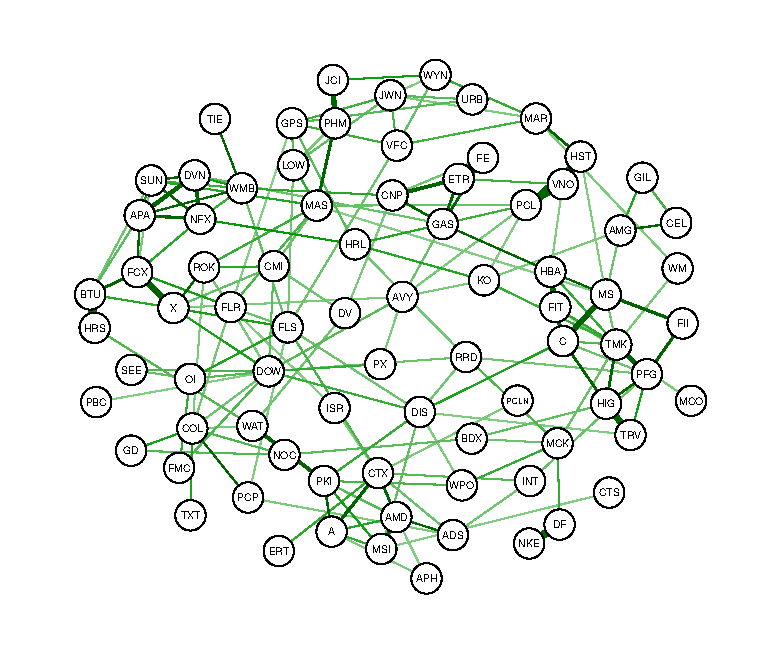
\includegraphics[scale=.9]{pics/stocks_mtp2}	
\end{center}
\end{frame}

%\begin{frame}{Sparsistency}
%Does such a procedure lead to a consistent estimation of the underlying graph? \alert{Of course not.}\\[.3cm]
%
%%For example if the true graph has no edges, the estimated graph will typically not be even very sparse. \\[.3cm]
%
%	Some regularization is needed, see also:
%	{\small
%	\begin{itemize}
%		\item Slawski, Hein, \textit{Estimation of positive definite M-matrices and structure learning for attractive Gaussian Markov random fields}, LAA, 2015. 
%		\item Egilmez, Pavez, Ortega, \textit{Graph Learning from Data under
%Structural and Laplacian Constraints}, 2017.
%%\item Egilmez, Pavez, Ortega, \textit{Learning Graphs with Monotone Topology
%%Properties and Multiple Connected Components}, 2018.\\[.5cm]
%	\end{itemize} }
%	\vspace{-.5cm}
%	\begin{block}{}
%		\textbf{Proposition}: M-matrices are closed under thresholding.
%	\end{block}
%\end{frame}



%\begin{frame}[plain,noframenumbering]{}
%\begin{center}
%	{\huge \textcolor{DarkRed}{Ferromagnetic Ising model}}
%\end{center}
%\end{frame}
%

%\begin{frame}{$\mtp$ exponential families}
%\begin{itemize}
%\item  
%$p(x;\theta)=g(x)\exp(\langle \theta,T(x)\rangle -A(\theta))$\\[.1cm]
%\begin{itemize}
%\item $T:\,\cX\to \R^{d}$\\[.1cm]
%\item $\cK=\{\theta:\, \int \exp(\langle \theta,T(x)\rangle)\nu({\rm d}x)<\infty\}$\\[.6cm]
%\end{itemize}
%%\item The following sets are convex
%%\begin{itemize}
%%\item $C$ = the set of canonical parameters
%%\item $K={\rm conv}(T(\cX))$ = the set of mean parameters  
%%\end{itemize}
%\item $\cK$ is convex and $A(\theta)$ is strictly convex in $\cK$
%\end{itemize}
%\vspace{-.1cm}
%%\pause
%\begin{block}{}
%\textbf{Theorem}:  The set of all $\theta\in \cK$ such that $p(x;\theta)$ is $\mtp$ is a relatively closed \textcolor{red}{convex} subset of $\cK$. 
%%In many interesting cases $\cC$ is a \textcolor{blue}{polyhedral}    cone.
%\end{block}
%%Proof of the first statement:	Let $\theta=(1-t)\theta_1+t\theta_2$, where $\theta_1,\theta_2$ lead to $\mtp$ distributions. Then\\[.2cm]
%%	$p(x;\theta)=\left( p(x;\theta_1)\right)^{1-t}\left( p(x;\theta_2 )\right)^{t}\exp\{(1-t)A(\theta_1)+tA(\theta_2 ) -A(\theta )\}$	
%%Proof: Define $\Delta_{x,y}(\theta)=\log\left(\tfrac{p(x\vee y;\theta) p(x\wedge y;\theta)}{p(x;\theta)p( y;\theta)}\right)$, then
%%$$
%%\Delta_{x,y}(\theta)=\langle\theta,T(x\vee y)+T(x\wedge y)-T(x)-T(y)\rangle+{\rm const}.
%%$$
%%So $\Delta_{x,y}(\theta)\geq 0$ for all $x,y$ defines a convex subset of $\cK$.
%\end{frame}

%\begin{frame}{$\mtp$ exponential families}
%\end{frame}

%\begin{frame}{Dependence on $g(x)$}
%\begin{block}{}
%\begin{itemize}
%	\item Proposition: The $\mtp$ property does not depend on the base measure. The counting/Lebesgue measure can be replaced by any other \alert{product} measure.  
%\end{itemize}	
%\end{block}
%\begin{itemize}
%	\item Remark: If the exponential family contains a product distribution then it can be chosen to be the base measure. \begin{itemize}
%	\item $\theta\in \cK$ is $\mtp$ if and only if  $F(x)=  -\langle\theta,T(x)\rangle$ is submodular.
%	\item also \alert{$\cC$ is a cone}.\\[.4cm]
%	\end{itemize}
%	\item If $F$ is twice differenciable then equivalently: $$\left\langle \theta,\tfrac{\partial^2 T}{\partial x_i\partial x_j}\right\rangle \geq 0\mbox{ and all } i\neq j, x\in \cX.$$
%\end{itemize}
%\end{frame}



%\begin{frame}{Maximum likelihood estimation}
%\begin{block}{}
%	\begin{itemize}
%\item $x^{(1)},\ldots,x^{(n)}\in \cX$ independent sample;\quad $\bar T:=\tfrac{1}{n} \sum_i T(x^{(i)})$\\[.4cm]
%\item the log-likelihood function:\quad $\ell(\theta)=n\langle \theta,\bar T\rangle -nA(\theta)$\\[.4cm]
%\item $\ell$ strictly concave in $\cK$ and so the MLE is unique (if exists) 
%\end{itemize}
%\end{block}
%\begin{itemize}
%	\item Hence, $\mtp$ distributions also admit a unique maximizer.\\[.4cm] 
%	\item The MLE usually exists under \emph{much} weaker conditions on $n$. 
%\end{itemize}
%\end{frame}

%\begin{frame}{Geometry of the MLE}
%	\begin{itemize}
%		\item Let $\mathcal{S}$ denote the interior of $\textrm{conv}(T(\mathcal{X}))$.
%		\item The MLE exists in the EF if and only if $\bar T=\tfrac{1}{n} \sum_i T(x^{(i)})\in\mathcal{S}$.
%		\item Let $\cK_2=\cK\cap \cC$ and define $\cS_2=\cS+\cC^\vee$
%	\end{itemize}
%	\begin{block}{}
%		Theorem: The MLE of $\theta$ based on $\bar T$ exists in the $\mtp$ model if and only if $\bar T\in\mathcal{S}_2$. It is then equal to the unique element $\hat\theta = \nabla A (\hat{\sigma}) $ that satisfies
%\begin{enumerate}
%\item[(a)] Primal feasibility: \;$\hat\theta\in\mathcal{K}_2$
%\item[(b)] Dual feasibility: \quad$ \hat{\sigma}\in\mathcal{S}$ with $\bar T - \hat\sigma\in\mathcal{C}^\vee,$
%%\item[(c)] \alert{Stationarity of Lagrangian:} \, $\tr(S\hat\theta)= m$,
%\item[(c)] Complimentary slackness: \;\; $\langle \bar T - \hat{\sigma},\,\hat\theta\rangle= 0$.
%\end{enumerate}
%	\end{block}
%	\begin{itemize}
%		\item We do not need $\bar T\in \cS$. Enough that $\bar T- u\in \cS$ for some $u\in \cC^\vee$.
%	\end{itemize}
%\end{frame}
%
%\begin{frame}{Binary distributions}
%	\begin{itemize}
%	\item Consider distributions $p(x)$ for $x\in \cX=\{0,1\}^n$.
%%		\item Canonical parameters: $\theta(x)=\log p(x)-\log p(\bs 0)$ .
%%		\item Sufficient statistic: For $x\in \cX$, define a vector $T(x)\in \{0,1\}^{\cX}$ such that $T(x)(y)=1$ if $x=y$ and it is zero otherwise.
%%		\item $\langle \theta,T(x)\rangle=\sum_{y\in\cX} \theta(y)T(x)(y)$.
%	\end{itemize}
%	\begin{itemize}
%		\item $\cS$ is the interior of the probability simplex so the MLE for binary distributions exists if and only if $\hat p(x)>0$ for all $x$. 
%	\end{itemize}
%	\vspace{-.3cm}
%	%\pause
%	\begin{block}{}
%		The MLE for $\mtp$ binary distributions if and only if both $\mathbf 0$ and $\mathbf 1$ are observed at least once, or in other words, 
%$$
%\mathcal S_2=\{p\in \Delta:\, p(\mathbf 0)>0, p(\mathbf 1)>0\}.
%$$
%Therefore, whenever $n\geq 2$, the MLE exists with a positive probability probability
%$$
%1-(1-p_{\mathbf 0})^n-(1-p_{\mathbf 1})^n+(1-p_{\mathbf 0}-p_{\mathbf 1})^n.
%$$	
%	\end{block}
%\end{frame}

%\begin{frame}{Pairwise interaction models}
%\begin{itemize}
%\item \textcolor{blue}{Pairwise interaction model} for a graph $G=(V,E)$
%$$
%p(x)=\tfrac{1}{Z}\prod_{i\in V}\psi_{i}(x_{i})\prod_{(i,j)\in E}\psi_{ij}(x_{i},x_{j})\quad\mbox{for all }x\in \cX.
%$$
%\end{itemize}
%\begin{block}{}
%\textbf{Proposition}: $p$ is $\mtp$ iff $\psi_{ij}$ are $\mtp$ functions.
%\end{block}
%\begin{itemize}
%\item e.g. ferromagnetic Ising model
% $$\psi_{ij}(x_i,x_j)=\exp(J_{ij}x_i x_j),\qquad J_{ij}\geq 0.$$
%% \item Gaussian graphical models $\theta_{ij}=K_{ij}$ with $K_{ij}\leq 0$
%\end{itemize}
%\end{frame}

%\begin{frame}{Symmetric Ising model}
%	The Ising model \emph{with no external field} 
%	$$
%	p(x)\;=\;\tfrac{1}{Z(J)}\exp\left(\sum_{uv\in E} J_{uv}x_ux_v\right)\quad x\in \{-1,1\}^{V}.
%	$$
%	\begin{block}{}
%	\begin{itemize}
%		\item Ferromagnetic if $J\geq 0$.
%		\item The covariance not necessarily an inverse  M-matrix.
%	\end{itemize}
%	\end{block}
%\end{frame}

%\begin{frame}{The normalizing constant}
%$$
%Z(J)\;=\;\sum_{x\in \cX} \prod_{uv\in E}\exp(J_{uv}x_u x_v)
%$$
%Useful identity
%$$
%\exp(J_{uv}x_u x_v)\;=\;\cosh(J_{uv})\Big(1+x_u x_v \tanh(J_{uv})\Big)
%$$
%and the fact that $x_v^{2}=1$ give
%$$
%Z(J)\;=\;2^{|V|}\prod_{uv\in E}\cosh(J_{uv})\sum_{E'\subset {\rm even}(G)}\prod_{uv\in E'}\tanh(J_{uv})
%$$
%\end{frame}
%
%\begin{frame}{Two special cases}
%	\begin{block}{}{\small
%		$$
%Z(J)\;=\;2^{|V|}\prod_{uv\in E}\cosh(J_{uv})\sum_{E'\subset {\rm even}(G)}\prod_{uv\in E'}\tanh(J_{uv}).
%$$}
%	\end{block}
%	\begin{itemize}
%		\item $G$ tree; ${\rm even}(G)=\{\emptyset\}$ $$Z(J)=2^{|V|}\prod_{uv\in E}\cosh(J_{uv})$$
%		\item $G$ n-cycle; ${\rm even}(G)=\{\emptyset,G\}$ $$Z(J)=2^{|V|}\prod_{uv\in E}\cosh(J_{uv})\Big(1+\prod_{uv\in E}\tanh(J_{uv})\Big)$$
%	\end{itemize}
%\end{frame}
%
%
%\begin{frame}{Edge covariances}
%Standard exponential families theory gives
%	$$\Sigma_{ij}\;=\;\E X_i X_j\;=\;\tfrac{\partial}{\partial J_{ij}}\log Z(J)$$
%	\vspace{.5cm}
%	
%	For example, if $G$ is an n-cycle
%$$
%\Sigma_{ij}\;=\;\tfrac{\tanh(J_{ij})+\prod_{uv\neq ij}\tanh(J_{uv})}{1+\prod_{uv\in E}\tanh(J_{uv})}
%$$
%\end{frame}
%
%\begin{frame}{Other covariances}
%\textbf{Proposition}:	If $G$ is an n-cycle 
%$$
%\Sigma_{ij}\;=\;\tfrac{\prod_{uv\in P_1}\tanh(J_{uv})+\prod_{uv\in P_2}\tanh(J_{uv})}{1+\prod_{uv\in E}\tanh(J_{uv})}
%$$
%\vspace{.5cm}
%
%This suggests some determinental representation.
%\end{frame}


%\begin{frame}{Treewidth $\leq 2$ graphs}
%	\textbf{Theorem} [Wermuth,Marchetti]: If $\Sigma$ is a covariance matrix in a symmetric Ising model over $G$ with treewidth $\leq 2$, then $(\Sigma^{-1})_{ij}=0$ for all $ij\notin E(G)$. \\[.3cm]
%	\begin{block}{}
%	Partial correlations \quad$\equiv$\quad conditional correlations		
%	\end{block}\vspace{.5cm}
%	\textbf{Theorem}: If $G$ has treewidth $\leq 2$ then for any $\mtp$ distribution in the corresponding symmetric Ising model $\Sigma$ is an inverse M-matrix. 
%\end{frame}
\begin{frame}[plain,noframenumbering]{}
\begin{center}
	{\huge \textcolor{DarkRed}{4.3 The binary Ising model}}
\end{center}
\end{frame}




\begin{frame}{Two psychological disorders, continued}
positive sample correlations but not $\mtp$
\begin{center}
\only<1>{The sample correlation:\\[.3cm]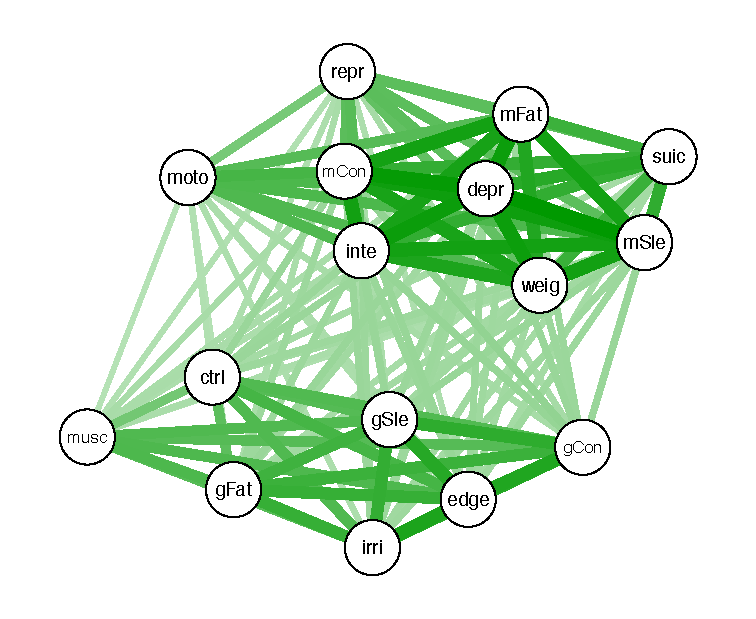
\includegraphics[scale=.6]{pics/scorrdepr}.}\only<2>{The $\hat J$ matrix:\\[.3cm]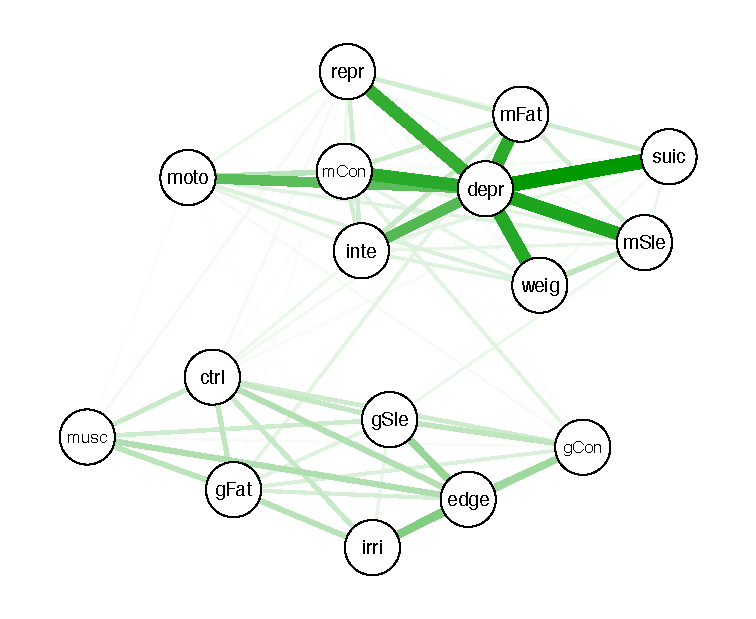
\includegraphics[scale=.6]{pics/Jdepr}}	
\end{center}
\vspace{-.6cm}
\only<1>{{\footnotesize Borsboom and Cramer, Network analysis: an integrative approach to the\\[-.2cm] structure of psychopathology, Annual review of clinical psychology, 9 (2013). }}
\only<2>{{\footnotesize Borsboom and Cramer report a similar picture obtained after asking 12 Dutch\\[-.2cm] clinicians for causal relationships!}}
\end{frame}

\begin{frame}[fragile]{Using \texttt{MTP2binary} package}
The Gaussian can be estimated using \texttt{MTP2binary} package.
The binary Ising model can be estimated using the \texttt{MTP2binary} package.
	\begin{lstlisting}
library(MTP2binary)
ncsdata=read.table(file="../DepressionAnxiety.txt") #read in data
colnames(ncsdata)=c("depr", "inte", "weig", "mSle", "moto", "mFat", "repr", "mCon", "suic", "anxi", "even", "ctrl", "edge", "gFat", "irri", "gCon", "musc", "gSle") #Define variable names.
XX <- as.matrix(ncsdata)
colnames(XX)=c("depr", "inte", "weig", "mSle", "moto", "mFat", "repr", "mCon", "suic", "anxi", "even", "ctrl", "edge", "gFat", "irri", "gCon", "musc", "gSle") #Define variable names.
# remove two variables that are perfectly correlated with each other
X <- 2*(XX[,-(10:11)])-1.   # and change to -1/1 coding
n <- nrow(X); d <- ncol(X)
# compute the second moments matrix and the mean vector
M <- t(X)%*%X/n
xbar <- apply(X,2,mean)
p0 <- mtp2.quad.mle(xbar,M,tol=1e-4,maxit=1000) # will take half hour
	\end{lstlisting}
%	J0 <- compute.J(p0)
%rownames(J0) <- colnames(J0) <- colnames(X)
%lay <-averageLayout(J0,cor(X), layout = "spring", repulsion = 1)
%# this is the correlation graph of the data X
%qgraph::qgraph(cor(X),labels=colnames(X),layout=lay)
%# this is the MLE graph under the MTP2 constraint
%qgraph::qgraph(J0,labels=colnames(X),layout=lay)
\end{frame}

%\begin{frame}{Testing $H_0: J\geq 0$}
%	\begin{alertblock}{Split Likelihood Ratio test}
%		Randomly split the data matrix into $X_0,X_1$. \\[.3cm]
%		Let $\hat h_1, \hat J_1$ the unrestricted maxima for the Ising model under $X_1$. \\[.3cm]
%		Compute the likelihood function $\cL(h,J;X_0)$ and its constrained maximum $\hat h_0$, $\hat J_0$.\\[.3cm]
%		We reject the null if $$U_n \;:=\;\frac{\cL(\hat h_1,\hat J_1;X_0)}{\cL(\hat h_0,\hat J_0;X_0)}\;> \;\frac{1}{\alpha}.$$
%		Theorem: The split LRT controls the type I error at level $\alpha$, i.e. $\sup_{h,J\geq 0} \P_{\theta_0} (U_n>1/\alpha)\leq \alpha.$
%	\end{alertblock}
%
%\end{frame}

%
%\begin{frame}{US Senators voting network}
%	\centering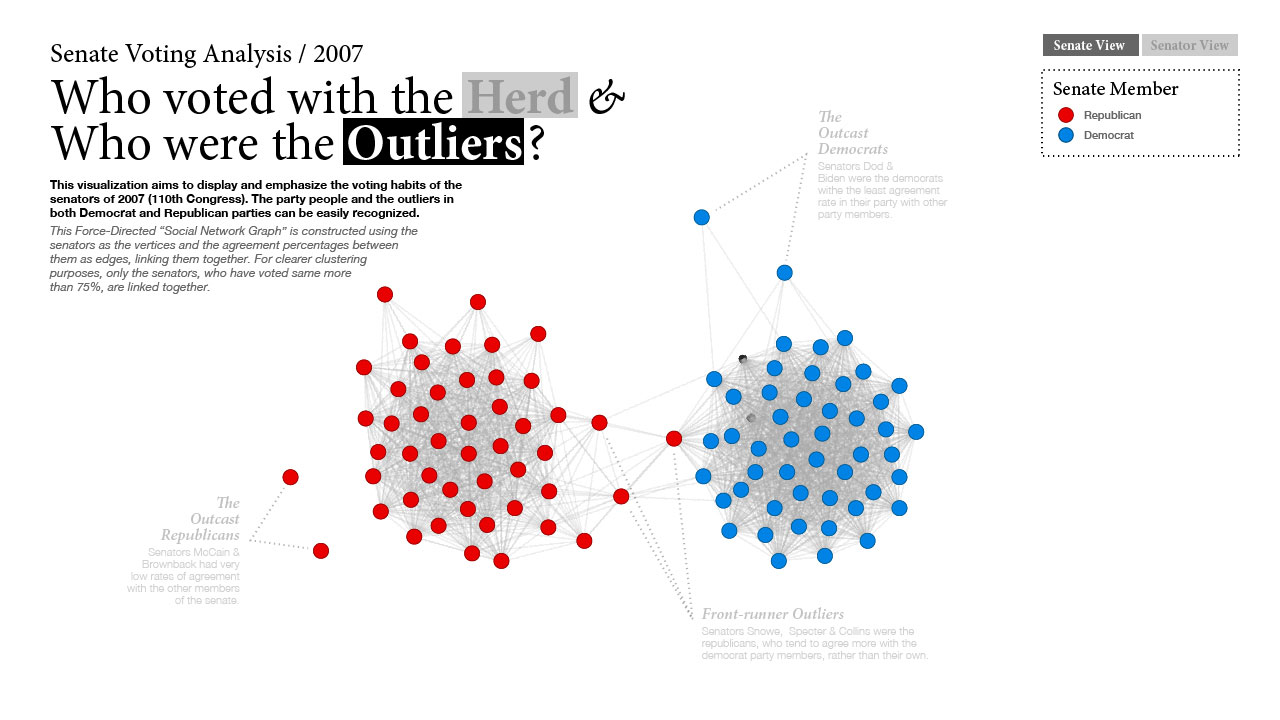
\includegraphics[scale=.28]{pics/ussenate.jpg}
%\end{frame}
%

\begin{frame}{Other interesting models/packages}
\texttt{mgm} - Estimation of k-Order time-varying Mixed Graphical Models and mixed VAR(p) models via elastic-net regularized neighborhood regression.\\[.2cm]
	\texttt{mixggm} - Mixtures of Gaussian graphical models for model-based clustering with sparse covariance and concentration matrices.\\[.2cm]
	\texttt{NetworkChange} - Network changepoint analysis for undirected network data.\\[.2cm]
	\texttt{graphicalVAR} - Estimates within and between time point interactions  using the Graphical VAR model in combination with regularization.\\[.2cm]
	\texttt{mlVAR} - Estimates the multi-level vector autoregression model on time-series data. Three network structures are obtained: temporal networks, contemporaneous networks and between-subjects networks.\\[.2cm]

\texttt{SparseTSCGM} - Computes sparse autoregressive coefficient and precision matrices for time series chain graphical models(TSCGM).\\[.3cm]
	\begin{beamercolorbox}[wd=\paperwidth,sep=5pt]{important}
	Related articles are on our reading list.	
	\end{beamercolorbox}

\end{frame}

\end{document}
